%!TEX root = thesis.tex
\chapter{Homeotropic nematics confined in toroids and bent capillaries}

\section{Introduction}
A system with broken reflection symmetry cannot be superimposed onto its reflection using only translations and rotations; it has a handedness and thus is chiral~\cite{RN175}.
Chirality can have important consequences for a system.
For example, as first shown by Pasteur~\cite{RN291}, a material's ability to rotate the polarization state of linearly polarized light results from broken reflection symmetry.
This phenomenon is called optical activity and the handedness of the system determines the rotation sense of the light polarization~\cite{RN291}.
Chiral systems can also exhibit ``structural color,'' where light interacting with a microscopic pattern produces color; for example, jeweled beetles appear iridescent due to light interacting with the chiral patterns on a beetle's exoskeleton~\cite{RN308,RN307}.
 % and can even be doped to form microlasers~\cite{RN305,RN306}.

Chiral systems can be formed from chiral building blocks, as in some photonic metamaterials~\cite{RN304,metameterial}, or chirality can emerge via spontaneous symmetry breaking in an achiral system~\cite{RN294}.
This latter scenario is often studied in nematic liquid crystals where the mesogens are achiral~\cite{RN297,RN296,RN298,RN295,RN299,RN193,RN24,RN192,RN191,RN293,RN302}.
Here, the symmetry-breaking is driven by the material elasticity; if the minimum energy state is chiral, then there must be a nontrivial twist distortion in the system.

This simplest way to break the reflection symmetry in a NLC is to prescribe twist with boundary conditions, as in the twisted nematic cell shown in Figure~\ref{f:4-SSB}(A).
In this scenario, the NLC is confined between two parallel plates with strong planar anchoring on each plate, specified by $\bm{\sigma}_1$ and $\bm{\sigma}_2$, respectively.
If the plates are in the $xy$-plane and the distance between them is $H$, then $\mathbf{n}(z = 0) = \bm{\sigma}_1$ and $\mathbf{n}(z = H) = \bm{\sigma}_2$.
When $\bm{\sigma}_1 \cdot \bm{\sigma}_2 = 0$, the boundary conditions require $\mathbf{n}$ to twist by $\pm \pi/2$ along a verical path.
Computing the free energy density for such a cell using a linear twist ansatz $\mathbf{n} = \hat{x} \cos (\tau z/H) + \hat{y} \sin(\tau z/H)$, with $\tau$ the twist angle of the director between the plates, we have:
\begin{align}
  f = K_{22}(\mathbf{n} \cdot \nabla \times \mathbf{n})^2 = K_{22}\tau^2/H^2,
\end{align}
In the cell shown in Figure~\ref{f:4-SSB}(A), $|\tau| = \pi/2$.
Following the director along $\hat{z}$, we see that the twist is counterclockwise and thus is called a left-handed (LH) twist.
However, the system could just as easily have a right-handed (RH) twist, as the spontaneous reflection symmetry breaking has no preference for either handedness in this case.
We also see that the amount of twist is set by the anchoring conditions, and is the same for any NLC provided the material obeys the boundary conditions.
However, if we were to change $\bm{\sigma}_1$ and $\bm{\sigma}_2$ such that $|\tau| \neq \pi/2$, the choice of handedness becomes biased; for example, if $\bm{\sigma}_1 \cdot \bm{\sigma}_2 = 1/\sqrt{2}$, then $\tau = \pi/4$ or $-3\pi/4$, leading to a difference in the free energy between the two twist directions.
Consequently, the system will have a greater probability to have $\tau = \pi/4$, since this twist corresponds to the minimum energy state.
\begin{figure}
  \centering
  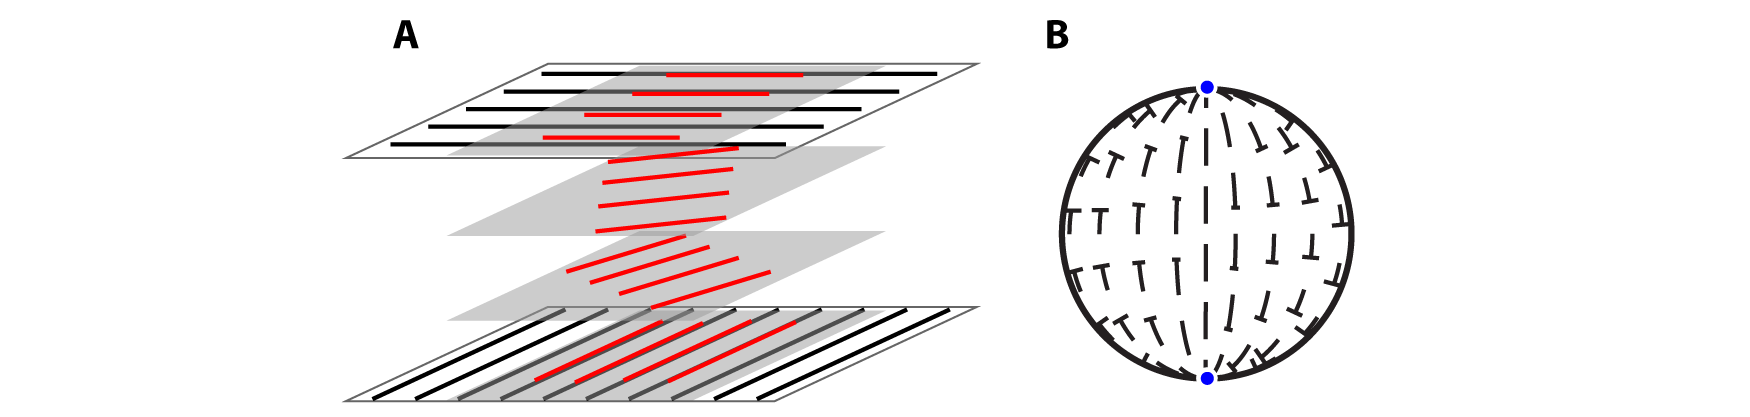
\includegraphics{figures/C4/Ch4-Figs_SSB.png}
  \caption{Spontaneous reflection symmetry breaking in twisted nematic cells and twisted bipolar droplets.
  (A), Schematic of a twisted nematic cell with a twist angle of $\pi/2$.
  The system could also satisfy the boundary conditions by twisting with the opposite handedness.
  (B), Schematic of a cross-section of the director in a twisted bipolar droplet.
  The nails represent the director going into the page.
  As with (A), the system could twist with the opposite handedness.}\label{f:4-SSB}
\end{figure}

If we want to explore scenarios where the NLC has equal probability to adopt either handedness with $|\tau| \neq \pi/2$, we need scenarios where more than one distortion is at play.
For example, consider a standard bipolar drop with degenerate planar anchoring, as shown schematically in Figure~\ref{f:2-OPMDrops}(A).
Here, there are both splay and bend distortions, and the structure is achiral.
If $K_{22}$ and $K_{33}$ are small enough compared to $K_{11}$, the bipolar drop will twist, [see Figure~\ref{f:4-SSB}(B)] relieving some of the splay distortions with the less costly twist and bend distortions~\cite{RN297,RN296,RN295}.
The criterion governing this instability is called the Williams criterion, $K_{11} > K_{22}+ 0.431 K_{33}$~\cite{RN297, williamsCrit}.
As with the twisted NLC cell with $|\tau| = \pi/2$, the handedness of the twist is randomly chosen.
Provided $K_{11}$, $K_{22}$, and $K_{33}$ satisfy the Williams criterion, the magnitude of the twist is determined by the elastic constants; in this scenario there is no way to tune the twist apart from changing the material properties of the NLC.

Prior work in our group with NLC confined to toroids with degenerate planar boundary conditions demonstrated that the amount of twist resulting from spontaneous symmetry breaking is not always only determined by the elastic constants~\cite{RN24}.
We found a doubly-twisted director configuration in toroidal droplets, where the magnitude of the twist grew with decreasing $\xi$.
Schematics of an achiral and of a doubly-twisted director field are shown in Figure~\ref{f:4-PlanarToroidsTwist}(A,B) and Figure~\ref{f:4-PlanarToroidsTwist}(C,D), respectively.
Under degenerate planar anchoring, the saddle-splay distortion drives the director at the interface to align along the smallest principle curvature of the interface according to Eq~\ref{e:2-K24SurfCouple}~\cite{RN59}.
For example, consider a cylinder with radius $a$ in the standard cylindrical coordinates $\{r, \theta, z \}$.
The principle curvatures are $\kappa_1 = -1/a$ along $\hat{\theta}$ and $\kappa_2 = 0$ along $\hat{z}$.
Thus, saddle-splay distortion will try to align the director along $\hat{\theta}$.

Increasing the difference between the principle curvatures of the interface will cause the system to twist more.
In our cylindrical example, this corresponds to decreasing $a$.
For a torus, we have another option.
In the $\{r, \theta, \varphi\}$ toroidal coordinates defined schematically in Figure~\ref{f:3-EqDefs}(B), we can write the two principle curvatures:
\begin{align}
  \kappa_1 &= -\frac{1}{a} \\
  \kappa_2(\theta) &= \frac{\cos(\theta)}{a(\xi-\cos(\theta))},
\end{align}
Thus, decreasing $\xi$ in our toroidal droplets causes $|\kappa_1-\kappa_2(0)| = \xi/(a(\xi-1))$ to increase, leading to our observations of increasing twist with decreasing $\xi$, as shown by the (${\color{red} \bullet}$) symbols in Figure~\ref{f:4-PlanarToroidsTwist}(E).

However, the twist still depends on the elastic constants.
This is easiest to see by considering the Frank-Oseen free energy of a linear double-twist in the $\xi \rightarrow \infty $ ``cylindrical limit'' of a torus.
Here, we use the ansatz in toroidal coordinates:
\begin{equation}\label{e:4-planransatz}
\mathbf{n} = \hat{\theta}\frac{\omega r}{a-g \frac{r}{\xi} \cos \theta} + \hat{\varphi}\sqrt{1 - \left ( \frac{\omega r}{a-g \frac{r}{\xi} \cos \theta} \right )^2 },
\end{equation}
where $\omega$ and $g$ are parameters that determine the amount of twist and splay in the director field, respectively; $g=1$ corresponds to a splay-free configuration.
The free energy per unit length in this limit is given by:
\begin{equation}\label{e:4-FEPlanarTwist}
  \frac{F}{2 \pi K_{33}} = \frac{K_{22}-K_{24}}{K_{33}}\omega^2 + \frac{\omega^4}{4} + \frac{K_{22}}{K_{33}}\sum\limits_{n=3}^{\infty} \frac{\omega^{2n}}{2n}.
\end{equation}
For $\omega \ll 1$, we can ignore the higher-order terms in the summation and minimize F to obtain:
\begin{equation}
  \omega = 0 ; \quad \omega = \pm \sqrt{2\frac{K_{24}-K_{22}}{K_{33}}}.
\end{equation}
In this case $\omega = 0$ corresponds to a maximum in $F$.
The twist angle is obtained by considering the angular difference between $\mathbf{n}(r=a, \theta = \pi/2)$ and $\mathbf{n}(r = a,\theta = 3\pi/2)$:
\begin{align}
  \tau &= \arccos(\mathbf{n}(r=a, \theta = \pi/2) \cdot \mathbf{n}(r = a,\theta = 3\pi/2)) \nonumber \\
       &= \arccos(1-2\omega^2) \nonumber \\
       &= \arcsin(2 \omega \sqrt{1 + \omega^2}) \nonumber \\
       &= 2\arcsin(\omega).
\end{align}
Clearly then, the system will break reflection symmetry when $K_{24}> K_{22}$, and $|\tau|$ increases with increasing $K_{24}$ and decreasing $K_{22}$.
\begin{figure}
  \centering
  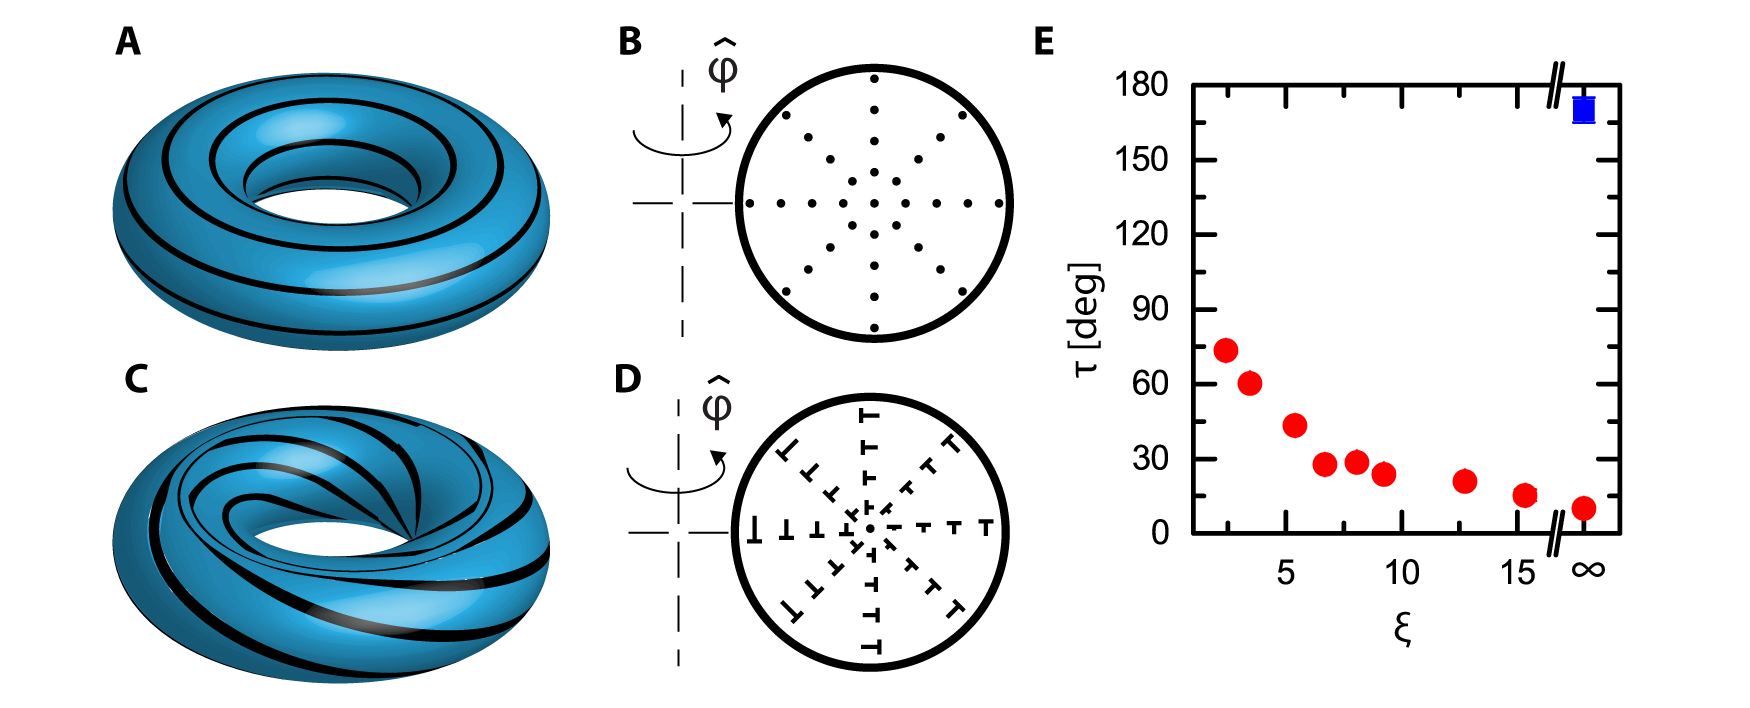
\includegraphics{figures/C4/Ch4-Figs_PlanarTwist.png}
  \caption{NLC in toroids with degernate planar anchoring has a doubly-twisted ground state.
  (A-D), Director schematics for nematic toroids with degenerate planar anchoring.
  (A,B) Schematics for the twist-free state with (A) showing the director at the surface and (B) showing the director in a cross-section of the tube.
  (C,D) Schematics for doubly-twisted state with (C) showing the director at the surface and (D) showing the director in a cross-section of the tube.
  The nails represent the director going into the page.
  (E) Twist angle measured through the tube $\tau$ vs aspect ratio $\xi$ for (${\color{red} \bullet}$) 5CB and (${\color{blue} \blacksquare}$) SSY confined to toroidal droplets and cylindrical geometries.
  $\xi = \infty$ corresponds to measurements in a cylindrical geometry, and $\xi < \infty$ are previously published data in toroidal droplets from Ref.~\cite{RN24}.}\label{f:4-PlanarToroidsTwist}
\end{figure}

We~\cite{RN293} and others~\cite{RN191} explored this directly by confining a Lyotropic Chromonic Liquid Crystal (LCLC) to a cylindrical capillary under degenerate planar anchoring conditions.
LCLC are an aqueous dispersion of plank-like molecules that self-assemble into columnar aggregates; these aggregates then form a nematic at appropriate temperature and concentration~\cite{RN303}.
In the nematic phase, LCLC typically have $K_{11} \sim K_{33} \sim 10 K_{22}$; in the capillary, the small $K_{22}$ yielded measured values of $|\tau| \approx 170 ^{\circ}$ for the LCLC Sunset Yellow (SSY).
For comparison, using the value of $K_{22}/K_{33}=0.4$ for 5CB and the value of $K_{24} = (1.02 \pm 0.02) K_{22}$ measured from our experiments with 5CB confined to toroidal droplets under degenerate planar anchoring, $|\tau (\xi \rightarrow \infty)| = 15^{\circ} \pm 15^{\circ}$.
We verify the twist in this limit directly using 5CB confined to a cylindrical geometry and find $|\tau (\xi = \infty)| = 9^{\circ} \pm 1^{\circ}$.
In fact, in our experiments, even when $\xi \sim 1$, we never measured $|\tau| > 80^{\circ}$.
We place these measurements of (${\color{blue} \blacksquare}$) SSY and (${\color{red} \bullet}$) 5CB in cylindrical geometries on the twist-angle plot in Figure~\ref{f:4-PlanarToroidsTwist}(E).
Thus, even though saddle-splay lets us tune chirality via geometry, there is still a large influence from the material constants.

Inspired by these results in planar-anchored nematic toroids and capillaries, in this Chapter we consider a 5CB confined to a toroidal droplet under homeotropic anchoring.
For homeotropic anchoring, the saddle-splay contribution to the free energy is always a constant.
Despite the fact that the saddle-splay distortion does not enter into the energy minimization problem for homeotropic nematics, we find spontaneous reflection symmetry breaking and geometrically-controlled chirality.
Prior results for NLC with $K_{11}\sim K_{22} \sim K_{33}$ confined under homeotropic anchoring to capillaries~\cite{RN179} and to toroids with $a \sim \mathcal{O}(1)$ $\upmu$m~\cite{RN274} found an escaped-radial (ER) configuration as the ground state.
In contrast, when $K_{11}\sim K_{33} \gg K_{22}$, the system breaks reflection symmetry, and adopts a twisted-escaped-radial (TER) configuration~\cite{RN192}.
This was again observed using LCLC; as in the degenerate-planar case, the low $K_{22}$ results in a very large total twist.

What we find here is that confining a NLC with $K_{11}\sim K_{22} \sim K_{33}$ under homeotropic anchoring to toroidal droplets with $a \sim \mathcal{O}(100)$ $\upmu$m yields a TER configuration, where the total twist decreases with increasing $\xi$, similar to our previous findings in planar anchored toroids.
We attribute the twist to the additional bend distortion introduced as $\xi$ decreases.
This additional bend distortion is relieved by a twist distortion with a spontaneously-chosen handedness.
Our work demonstrates that geometry can tune chirality, even in the absence of an explicit curvature-coupling term in the free energy.

The rest of this Chapter is organized as follows.
We begin with an overview of the ER and highly-twisted TER configurations in cylindrical capillaries, discussing qualitative differences between the structures and establishing an intensity ratio as a qualitative way to distinguish between the two configurations.
We then consider NLC confined with homeotropic anchoring to toroidal droplets with $a \sim \mathcal{O}(100)$ $\upmu$m.
At low $\xi$ we see an intensity ratio similar to the intensity ratio from the high-twist TER capillaries, while at high $\xi$ we see an intensity ratio comparable to that from the achiral ER capillaries.
Next, we use Jones Calculus to simulate OPM textures for a given director field, and validate our implementation on well-studied director configurations in spheres.
We use a linear double-twist ansatz in a torus to demonstrate technical details of our implementation.
Furthermore, we establish that we can successfully simulate OPM textures from twisted director fields by comparing the measured twist angle in our simulations with the twist angle imposed by the given director field.
We also simulate TER textures in toroids and capillaries, finding that the intensity ratio decreases as the twist increases.
Since this relationship is monotonic, the simulations indicate that comparing the intensity ratio in different toroids serves as a proxy for comparing the amount of twist in the toroids.
Finally, we confirm that the twist is driven by the local geometry by confining NLC to bent capillaries under homeotropic anchoring.
We measure a local aspect ratio and find that the intensity ratio in the bent capillaries has the same behavior as the intensity ratio in our homeotropic toroids.
This implies that we can tune chirality with confining geometry, even in the absence of the saddle-splay distortion that directly couples the director at the surface with the curvature of the surface.




\section{Escaped radial and twisted escaped radial configurations in capillaries}
Consider NLC confined to a cylindrical capillary under homeotropic boundary conditions; in cylindrical coordinates $\{r,\theta,z\}$, we specify the boundary conditions with $\mathbf{n} = \hat{r}$ at the boundary.
Restricting ourselves to a radial director field, $\mathbf{n} = \hat{r}$ everywhere, there is an $s = +1$ line defect running along $\hat{z}$ at the center of the capillary, as shown in Figure~\ref{f:4-EscapeSchem}(A).
However, recall from Chapter~\ref{c:2-defects} that integer-strength disclination lines are not topologically stable in a 3D NLC.
Similar to line defects in 2D nematics or wall defects in 3D nematics, the singular $s = +1$ distortion can be continuously deformed to form a nonsingular distortion, as shown in Figure~\ref{f:2-Smearing}~\cite{RN179,RN290,RN289}.
As illustrated in Figure~\ref{f:4-EscapeSchem}(B), the radial director field ``escapes into the third dimension'', such that  $n_{z} \neq 0$, hence the name escaped-radial.
In the one-constant approximation, the ER director field is analytically solvable, with $\mathbf{n} = \{\sin(\Omega),0,\cos(\Omega)\}$, where $\Omega(r) = 2 \arctan(r/a)$ gives the director angle measured off of $\hat{z}$, with $a$ the cylinder radius, as shown by the blue curve in Figure~\ref{f:4-EscapeSchem}(D)~\cite{RN179,RN290}.
Provided $a \gtrsim 0.1$ $\upmu$m, the ER configuration is the ground state solution~\cite{RN194}; the costly splay distortion in the vicinity of the singular line is relieved by a less-costly bend distortion, with the cost of the bend distortion increasing as $a$ decreases.
When $a \lesssim 0.1$ $\upmu$m, the cost of the bend distortion in the escape is too great and the $s = +1$ line defect is energetically stable.
For NLC where $K_{11} \neq K_{33}$, $\Omega(r)$ changes~\cite{RN321}.
When $K_{11} \ll K_{33}$, the $n_z$ component of the director only becomes appreciable when $r \approx 0$.
Hence, when $K_{11} < K_{33}$ we say that the director escapes more gradually, or slower.
In contrast,  when $K_{11} \gg K_{33}$, the $n_z$ component becomes appreciable for $r \approx a$; when $K_{11} > K_{33}$ we say that the director escapes more abruptly, or faster.
These behaviors can be visualized by taking $\Omega(r) = (\pi/2)(r/a)^{\phi}$, where $\phi < 1$ produces a slower escape and $\phi > 1$ produces a faster escape [red contours, Figure~\ref{f:4-EscapeSchem}(D)].
The $\phi = 1$ behavior is similar to the escape in the 1-constant approximation [blue line, Figure~\ref{f:4-EscapeSchem}(D)].
\begin{figure}
  \centering
  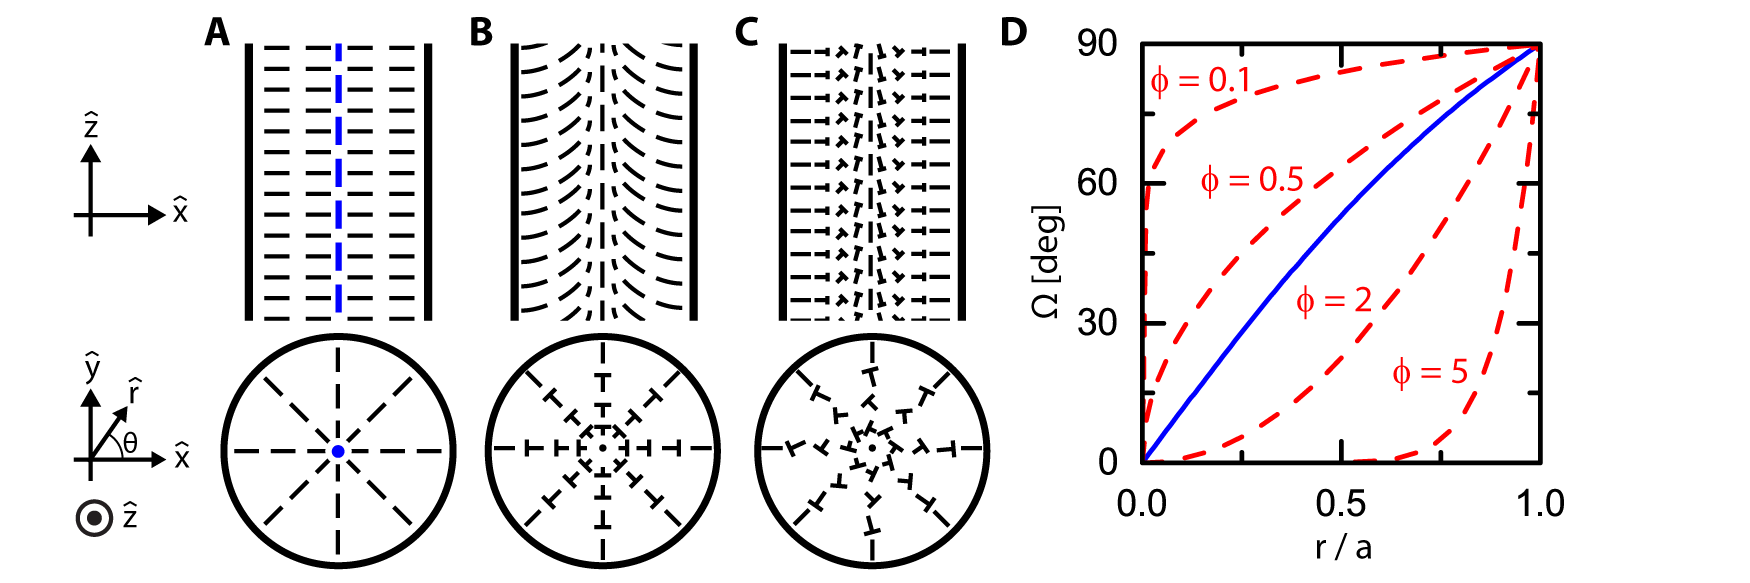
\includegraphics{figures/C4/Ch4-Figs_EscapeSchem.png}
  \caption{Singular and escaped-radial distortions in cylindrical geometries.
  (A-C), Cross-sections showing the director fields for a (A) singular $s = +1$ distortion, a (B) escaped-radial distortion, and a (C) twisted escaped-radial distortion.
  The nails represent the director going into the page.
  (D), Director angle $\Omega$ measured off of the cylinder axis as a function of normalized radius, $r/a$, with $a$ the cylinder radius. The blue curve corresponds the equilibrium solution for the 1-constant approximation, while the red curves correspond to $\Omega = (\pi/2)\,(r/a)^{\phi}$, with $\phi = 0.1,0.5,2,5$.
  The curves with $\phi = 0.1,0.5$ escape slower than the equilibrium solution, while the curves with $\phi = 2, 5$ escape faster than the equilibrium solution.}\label{f:4-EscapeSchem}
\end{figure}

Now with an ER configuration in the 1-constant approximation, let $K_{22}$ vary while keeping $K_{11} = K_{33} = K$.
When $K_{22} \lesssim 0.27K$~\cite{RN192}, the system can relieve some of the bend and splay distortions in the ER configuration by twisting, yielding the twisted escaped-radial configuration shown in Figure~\ref{f:4-EscapeSchem}(C), where now $\mathbf{n}$ has components along $\hat{r}$, $\hat{\theta}$, and $\hat{z}$.
This configuration was first observed using LCLC~\cite{RN192}.
Since $K_{22} \sim 10^{-1}K$ for LCLCs, they frequently exhibit spontaneous reflection symmetry breaking~\cite{RN192,RN191,RN293,RN193,RN302}.


\subsection{Intensity profile and intensity ratio}
We fill cylindrical capillaries with either 5CB or with a 31.5\% w/w aqueous solution of SSY; at this concentration, SSY is in the nematic phase~\cite{RN303}.
We use capillaries that are at least 4 cm long with diameters from $50$ $\upmu$m to 400 $\upmu$m.
To enforce homeotropic anchoring for the 5CB-filled capillaries, we first fill the capillary with $0.1\%$ w/w lecithin in hexane and then let the hexane dry, depositing the lecithin on the inner surface of the capillary.
We check each capillary with a microscope to make sure that the hexane has fully evaporated; this process can take anywhere from 10 minutes for the largest diameter capillaries to several hours for the smallest capillaries.
For the SSY-filled capillaries, the capillaries were coated with parylene using chemical vapor deposition.
The work was done by Karthick Nayani and Rui Chang using a commercial parylene coater (PDS2010; Specialty Coating Systems) according to a previously published protocol~\cite{RN192}.
The precurser, [2,2]paracyclophane, was vaporized at 160$^o$ C, pyrolized into monomer at 650$^o$ C, and deposited at 20$^o$ C; the entire process was performed under vacuum (~55 mtorr).

Bright-field images, shown in Figure~\ref{f:4-StraightCaps}(A,C), depict a 5CB and a SSY capillary, respectively.
The corresponding OPM images are shown in Figure~\ref{f:4-StraightCaps}(B,D); from previous results, we expect the configurations to be ER and TER, respectively~\cite{RN179,RN192}.
By eye, it is easy to see that the OPM textures shown in Figure~\ref{f:4-StraightCaps}(B,D) are different; this makes sense when we consider the director field in each configuration and its impact on the intensity profile across the capillary.
When the polarizer and analyzer (PA) are aligned along $\hat{z}$ and $\hat{x}$, an OPM texture of an ER capillary [Figure~\ref{f:4-StraightCaps}(B)] should have three regions of extinction corresponding to the regions near the boundary and to the center of the capillary.
In these regions, $\mathbf{n}$ is along the P or A direction.
Between these three dark regions there are two bright regions, corresponding to locations where $\mathbf{n}$ has components along both $\hat{x}$ and $\hat{z}$.
This dark-bright-dark-bright-dark pattern is the signature of an ER capillary; now plotting the intensity profile across the capillary in Figure~\ref{f:4-StraightCaps}(E), we see that there are two clear intensity peaks corresponding to the bright regions, and an intensity minimum in the middle of the profile corresponding to the dark central region.
Note that the intensity minimum is greater than zero; we believe this is due to scattering from thermal fluctuations in the director~\cite{RN33}.
\begin{figure}
  \centering
  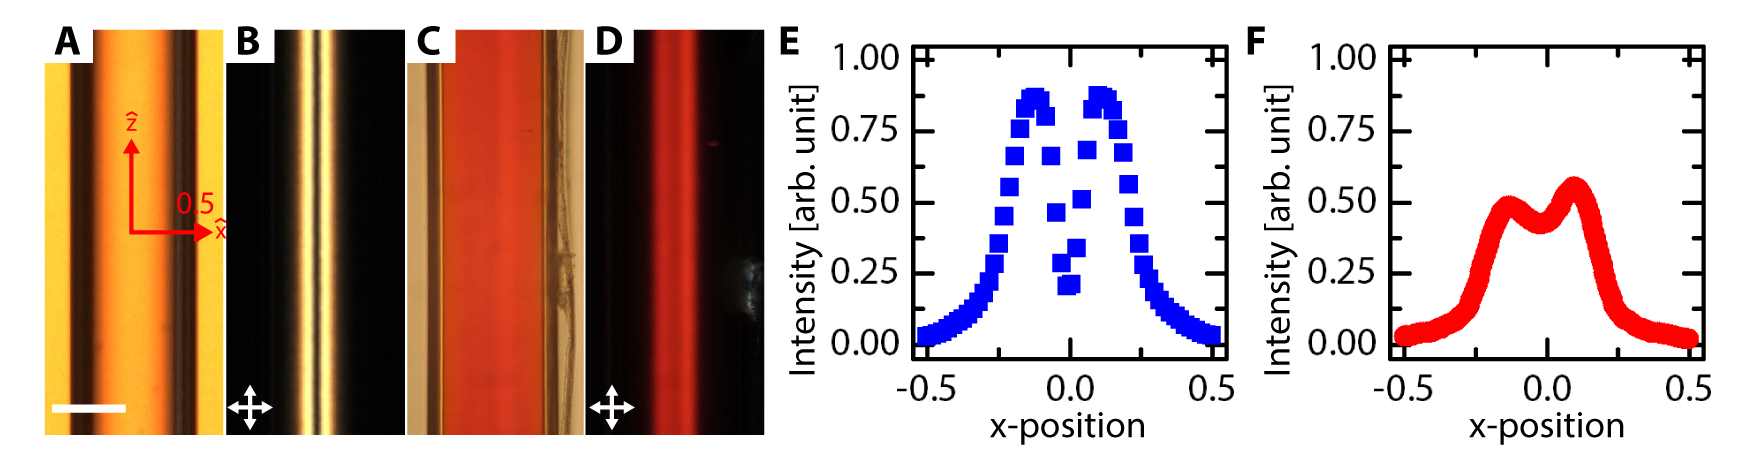
\includegraphics{figures/C4/Ch4-Figs_StraightCaps.png}
  \caption{ER and TER capillaries and intensity profiles.
  (A,C), Bright field images of a capillary filled with (A) 5CB and (C) SSY with homeotropic anchoring.
  (B,D), corresponding OPM images showing that (A,B) 5CB has an ER configuration and (C,D) SSY has a TER configuration.
  (E,F), Intensity profiles measured across the capillary for (E) the 5CB texture in (B), and (F), the SSY texture in (D). The intensity scale is the grayscale intensity, with $1$ corresponding to the white and $0$ to black.}\label{f:4-StraightCaps}
\end{figure}

Conversely, when we look at the OPM texture for a TER configuration [Figure~\ref{f:4-StraightCaps}(D)], we see that the central region is no longer dark, but that it has an intensity comparable to the intensity of the two ``bright'' regions flanking the central region.
We can rationalize this by following the director schematic in Figure~\ref{f:4-EscapeSchem}(C) along $\hat{y}$ through the center of the capillary.
We see that the nonzero $n_{\theta}$ component results in $\mathbf{n}$ having components along both $\hat{x}$ and $\hat{z}$, the P and A directions, causing the transmitted intensity in this central region to grow [Figure~\ref{f:4-StraightCaps}(D)].
Plotting the intensity profile across the capillary in Figure~\ref{f:4-StraightCaps}(F), we see that there is still a central minimum surrounded by two peaks; however, the central minimum in the TER configuration is much higher than the central minimum in an ER configuration.
In addition, we see that the peaks in the intensity profile do not have the same intensity value.
This is a common feature of the TER profiles, and there is no trend in which side has a higher value.
We quantify each intensity profile with an intensity ratio $I_{max}/I_{min}$, with $I_{max}$ the average intensity of the two peaks flanking the central minimum and $I_{min}$ the intensity of the central minimum.
Our ER capillaries have $I_{max}/I_{min} \approx 4$ while our TER capillaries have $I_{max}/I_{min} \gtrsim 1$.
We check that this phenomenon is not dependent on the LC chosen by comparing with the intensity profile of an ER SSY capillary; while the ground state in a homeotropic SSY capillary is a TER configuration, just after being filled the SSY capillary has a transient ER configuration that spontaneously breaks reflection symmetry after a few minutes.
As with the ER textures from the 5CB capillaries, $I_{max}/I_{min} \approx 4$ in the transient ER SSY capillary.




\section{Nematic liquid crystals in toroids}
We make stable toroidal droplets as detailed in Chapter~\ref{c:3}, with 5CB as our inner liquid and an aqueous yield-stress material.
Our yield-stress material for homeotropic nematic toroids is similar to that used in our prior work with planar-anchored nematic toroids~\cite{RN24}, except here, we have replaced the polyvinyl alcohol used to enforce degenerate planar anchoring with sodium dodecyl sulfate (SDS) to enforce homeotropic anchoring.
The yield-stress material consists of (i) 1.5\% w/w polyacrylamide microgels (Carbopol ETD 2020), (ii) 30\% w/w Ethanol, (iii) 3\% w/w Glycerol, (iv) 25\% w/w 32 mM SDS in ultrapure water, and (v) 40.5\% w/w ultrapure water.
Thus, the final mixture has approximately 8 mM SDS, a concentration that yields strong homeotropic anchoring~\cite{RN235}.
To make the yield-stress material, we mix all the ingredients together, wait for $\sim 24$ hrs to allow the Carbopol to hydrate, and then neutralize the mixture by adding a volume of 2M NaOH solution until the pH$\approx 7$.
Neutralizing the dispersion causes the polyacrylamide microgels to swell, increasing both the yield-stress and the transparency~\cite{RN24,RN47}.

We view our toroidal droplets from the top under both bright-field and with crossed polarizers, as shown in Figure~\ref{f:4-HomeoToroidsExp}(A,D) and Figure~\ref{f:4-HomeoToroidsExp}(B,E), respectively.
In the OPM texture in Figure~\ref{f:4-HomeoToroidsExp}(B) for a toroid with $\xi = 5$, the regions where the tube of the torus is along the orientation of the polarizer and analyzer (P and A), the intensity pattern has the characteristic dark-light-dark-light-dark profile associated with an ER texture where the cylinder axis is oriented along the P and A directions.
However, for the toroid with $\xi = 1.8$, the OPM texture in Figure~\ref{f:4-HomeoToroidsExp}(E) has more of a spiral-like texture.
To quantify these patterns, we measure the intensity profile across the tube of the torus.
\begin{figure}
  \centering
  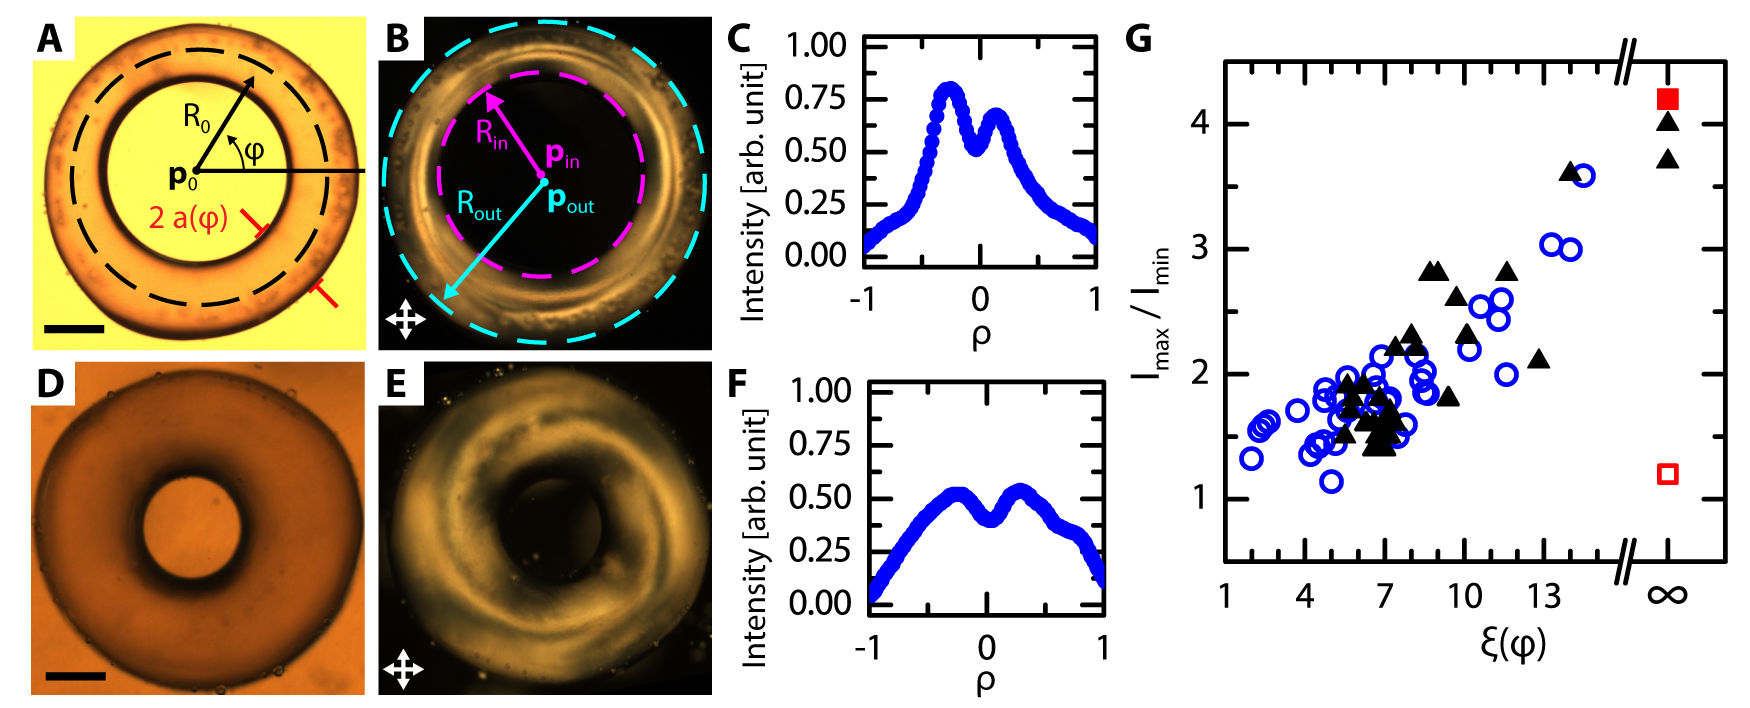
\includegraphics{figures/C4/Ch4-Figs_HomeoToroidsExp.png}
  \caption{Images and intensity ratios for homeotropic nematic toroids.
  (A,B,D,E), (A,D) Bright-field and (B,E) associated OPM textures for toroids with (A,B) $\xi = 5$ and (D,E) $\xi = 5$.
  The central circle, defined by the radius $R_{0}$, center $\mathbf{p}_0$, and polar angle $\varphi$, as well as the local tube radius $a(\varphi)$ are defined on the image in (A).
  The inner and outer circles, given by the radii $R_{in}$ and $R_{out}$ and centers $\mathbf{p}_{in}$ and $\mathbf{p}_{out}$, respectively, are drawn on the OPM texture in (B).
  (C,F), OPM Intensity profiles across the tube of the toroid in (B,E), respectively.
  These profiles are taken at $\varphi = 0$, with $\phi \in [-1,1]$ parameterizing the contour from the inner circle to the outer circle for the given $\varphi$.
  Both profiles show two maxima surrounging a central minimum.
  We take $I_{max}$ to be the average of the intensity values of the maxima and $I_{min}$ to be the intensity at the central minimum.
  (G), $I_{max}/I_{min}$ vs $\xi(\varphi) = R_0/a(\varphi)$ for a series of (${\color{blue} \circ}$) homeotropic 5CB toroidal droplets, (${\blacktriangle}$) homeotropic 5CB bent and straight capillaries, and (${\color{red} \blacksquare},\,{\color{red} \square}$) homeotropic SSY straight capillaries.
     (${\color{red} \blacksquare}$) corresponds to the transient ER state, while (${\color{red} \square}$) corresponds to the equilibrium TER state.
     Scale bars in (A,D) are 250 $\upmu$m.}\label{f:4-HomeoToroidsExp}
\end{figure}

\subsection{Measuring the intensity profile and aspect ratio}
From the top view, the azimuthal angle $\varphi$ in toroidal coordinates, $\{r,\theta,\varphi \}$ [see Figure~\ref{f:3-EqDefs}(B)], corresponds to the polar angle in a set of polar coordinates, $\{p,\varphi \}$, in the image itself.
As $\varphi$ is measured along the central ring of the torus, $\mathbf{p}_0 = (0,\varphi)$ corresponds to the center of the central ring of the torus in the image, as displayed on the bright-field image in Figure~\ref{f:4-HomeoToroidsExp}(A).
We take our intensity profiles in the OPM textures across the tube of the torus for a constant $\varphi$ from $p = R_0 - a(\varphi)$ to $p = R_0+ a(\varphi)$, where $R_0$ is the radius of the central ring of the torus and $a$ is the tube radius.
We parameterize each intensity profile with a variable $\rho = (p - R_0)/a(\varphi)$, such that $\rho \in [-1,1]$ corresponds to $p \in [R_0 - a(\varphi),R_0 + a(\varphi)]$.
We note that while for a perfect torus $a$ is constant, our toroidal droplets are not perfectly axisymmetric and thus $a$ has some $\varphi$-dependence.

We find the central ring, find $a(\varphi)$, and determine the intensity profiles with a custom MATLAB script.
We start by converting each image to grayscale using MATLAB's \texttt{rgb2gray} algorithm: $\mathit{gray} = 0.299 R + 0.587 G + 0.114 B$, where $R,G,B$ are the intensities in the red, green, and blue channels, respectively.
In the grayscale images, $1$ corresponds to white and $0$ to black.
From our top-view image, we start by selecting points along the inner and outer contours of the toroid in the image.
We then fit the points on each contour to a circle, giving us the radii $R_{in}$, $R_{out}$ and centers $\mathbf{p}_{in}$, $\mathbf{p}_{out}$ of the inner and outer contours, respectively.
Examples of these contours are drawn on the OPM texture in Figure~\ref{f:4-HomeoToroidsExp}(B).
Note how $\mathbf{p}_{in}$ and $\mathbf{p}_{out}$ in Figure~\ref{f:4-HomeoToroidsExp}(B) are close to each other but are not the same; this reflects the fact that we do not have a perfect torus.

For a given torus, we then take the average aspect ratio $\xi = R_0/a_{av} = (R_{out}+R_{in})/(R_{out}-R_{in})$, with the central ring radius $R_0=(R_{out}+R_{in})/2$ and the average tube radius $a_{av} = (R_{out}-R_{in})/2$.
We also calculate the origin of our polar coordinate system in the image, $\mathbf{p}_0 = (\mathbf{p}_{in}+\mathbf{p}_{out})/2$.
For a given $\varphi$, we take the intensity profile starting at the inner contour $|\mathbf{p}-\mathbf{p}_{in}| = R_{in}$ and increasing $p$ until we reach the outer contour $|\mathbf{p}-\mathbf{p}_{out}| = R_{out}$.
The length of this profile is $2 a(\varphi)$, allowing us to calculate a local aspect ratio $\xi(\varphi) = R_0/a(\varphi)$.
We then parameterize each intensity profile in terms of $\rho$; example profiles for $\varphi = 0$ for the OPM textures  in Figure~\ref{f:4-HomeoToroidsExp}(B,E) are shown in Figure~\ref{f:4-HomeoToroidsExp}(C,F), respectively.
These [Figure~\ref{f:4-HomeoToroidsExp}(C,F)] are typical intensity profiles for our homeotropic toroids, where we always take our intensity profiles with $\hat{\varphi}$ along either the P or A direction.
Like the intensity profiles of the TER capillaries [see Figue~\ref{f:4-StraightCaps}(F)], the maxima in the intensity profiles of our toroids do not always have the same value.
Similarly, there is no general trend in which maximum is larger.


\subsection{Large aspect ratio toroids}
We first look at our larger $\xi$ toroids [see Figure~\ref{f:4-HomeoToroidsExp}(A,B)]; the OPM texture resembles an ER texture and the intensity profiles [Figure~\ref{f:4-HomeoToroidsExp}(C)] show a central minimum flanked by two maxima.
However, we find that $I_{max}/I_{min} < 4$, with $4$ the value we observed in our ER capillaries.
In the example profile in Figure~\ref{f:4-HomeoToroidsExp}(C), $I_{max}/I_{min} = 1.45$ for $\xi(0) = 2.8$.
Thus, we hypothesize that our larger aspect ratio toroids have a TER configuration.
We emphasize that this twist occurs despite the fact that we have homeotropic anchoring.
With homeotropic anchoring, the saddle-splay distortion does not drive the formation of a twisted state, as it did in our previous work with NLC toroids with degnerate planar anchoring~\cite{RN24}.


\subsection{Small aspect ratio toroids}
When we look at toroids with smaller $\xi$, we initially see that the intensity pattern has changed to a spiral texture of alternating dark and light regions [Figure~\ref{f:4-HomeoToroidsExp}(E)], no longer so clearly resembling the dark-bright-dark-bright-dark texture of an ER or TER texture.
However, when we examine the intensity profile of the spiral textures, we still find qualitative similarities with the intensity profile of a TER configuration, with a central minimum surrounded by two maxima and $I_{max}/I_{min} < 4$.
For the example profile in Figure~\ref{f:4-HomeoToroidsExp}(F), $I_{max}/I_{min} =1.38$ and $\xi(0) = 2$.

For a series of toroids with different $\xi$ and $a$, we plot $I_{max}/I_{min}$ vs $\xi(\varphi)$ [(${\color{blue} \circ}$), Figure~\ref{f:4-HomeoToroidsExp}(G)] and find that $I_{max}/I_{min}$ increases with increasing $\xi(\varphi)$, approaching $I_{max}/I_{min} = 4$ as $\xi(\varphi) \gg 1$.
From this trend, we hypothesize that the twist in our TER toroids decreases as $\xi$ increases.
In order to both qualitatively investigate the role of twist in the intensity ratio as well as to test director configurations that could yield this spiral-like texture, we perform computer simulations of the OPM textures using Jones Calculus.




\section{Simulating polarized optical microscopy textures for twisted escaped radial director configurations}
\subsection{Jones Calculus and simulation details}
Jones Calculus is a method to describe and propagate polarized light through a birefringent material~\cite{RN232}.
The state of the polarized light is characterized by decomposing the electric field in the plane of polarization using a 2-dimensional Jones vector while neglecting the time dependence of the electric field.
We can neglect the time-dependence because while the electric field oscillates with time, the polarization state does not.
For example, allowing $\hat{x}$ to be horizontal, $\hat{y}$ to be vertical, and $\mathbf{k}_0 = \hat{z}$ the direction of the wavevector of the polarized incident light, we can write the normalized electric field as:
\begin{align}
\mathbf{E} &=  \hat{x}E_x e^{i \phi _x} + \hat{y} E_y e^{i \phi _y}\\  &= e^{i \phi _x} \left( \begin{array}{c} E_x \\E_y e^{i(\phi _y - \phi _x)}      \end{array} \right). \label{e:4-jonesdecomp}
\end{align}
Thus, the Jones vector for a horizontal polarization state, a $+45^{\circ}$ polarization state, and a right-handed circular polarization state can be written as $(1,0)$, $(1,1)/\sqrt{2}$, and $(1,i)/\sqrt{2}$, respectively.
We have normalized the Jones vectors, removing the absolute phase prefactor $e^{i \phi _x}$ from Eq.~\ref{e:4-jonesdecomp} as the polarization state is dependent on neither the absolute phase nor the magnitude of the vector.
Note, in particular, that the Jones vector for the right-handed circularly polarized light gives the normalized field $\mathbf{E} = \hat{x}E_x e^{i \phi _x} + \hat{y} E_y e^{i( \phi _x+\pi/2)}$, as we would expect.

In order to propagate a polarization state through an optical element, such as a half-wave plate or a phase retarder, we write each component of the Jones vector representing the transformed state $\mathbf{E}^{trans}$ as a linear combination of the components of the Jones vector representing the initial state $\mathbf{E}^{init} = E^{init}_{x}\hat{x}+E^{init}_{y}\hat{y}$:
\begin{align}
\mathbf{E}^{trans} = \left ( \begin{array}{c} E^{trans}_{x} \\ E^{trans}_{y} \end{array} \right ) &= \left ( \begin{array}{c} A E^{init}_{x} + B E^{init}_{y} \\ C E^{init}_{x}+ D E^{init}_{y} \end{array} \right ) \nonumber \\
&= \left ( \begin{array}{cc} A & B \\C & D \end{array} \right )\left ( \begin{array}{c} E^{init}_{x} \\ E^{init}_{y} \end{array} \right ) = \bm{\Theta} \mathbf{E}^{init},
\end{align}
where $\bm{\Theta}$ is our transformation operator, which can be written as a $2 \times 2$ Jones matrix.
To propagate a Jones vector through multiple optical elements, the Jones matrix for each element is applied to the initial Jones vector sequentially.
For a series of $N$ elements:
\begin{equation}
\mathbf{E}^{trans} = \bm{\Theta}_N \bm{\Theta}_{N-1} \cdots \bm{\Theta}_2 \bm{\Theta}_1\, \mathbf{E}^{init} = \prod\limits^N_{\nu=1} \bm{\Theta}_{\nu} \mathbf{E}^{init} = \bm{\vartheta} \mathbf{E}^{init},
\end{equation}
where $\bm{\vartheta}$ is the operator representing the Jones matrix for the entire system.
A list of some common optical elements represented as Jones matrices in the $xy$ basis are found in Table~\ref{t:4-jmats}.
\begin{table}
\caption{Jones calculus operators for common optical elements}
\begin{tabular}{|c|c|}
\hline
{\bf Optical Element} & {\bf Jones matrix} \\ \hline \hline
Linear polarizer with axis of transmission horizontal & $\begin{pmatrix}1 & 0 \\ 0 & 0 \end{pmatrix}$ \\ \hline
Linear polarizer with axis of transmission vertical &$\begin{pmatrix}0 & 0 \\ 0 & 1 \end{pmatrix}$ \\ \hline
Linear polarizer with axis of transmission at $\pm 45^o$ with the horizontal &$\frac{1}{2} \begin{pmatrix}1 & \pm 1 \\ \pm 1 & 1\end{pmatrix}$ \\ \hline
Right/left circular polarizer & $\frac{1}{2} \begin{pmatrix}
1 & \pm i \\ \mp i & 1
\end{pmatrix}$ \\
\hline
\end{tabular}\label{t:4-jmats}
\end{table}

For a general phase retarder with the optic axis along $\hat{y}$, the transformation operator is written as~\cite{RN232}:
\begin{equation}\label{e:4-fastaxisy}
\bm{\Theta} = \begin{pmatrix}e^{i \phi_x} & 0 \\ 0 & e^{i \phi_y} \end{pmatrix}.
\end{equation}
When the orientation of the optic axis is not along $\hat{y}$, we use a rotation matrix to rotate $\mathbf{E}^{init}$ and make it coincide with $\hat{y}$ so we can use Eq.~\ref{e:4-fastaxisy}; we undo our initial rotation with a second rotation matrix afterwards~\cite{RN310}:
\begin{equation} \label{e:4-jones_decouple}
\mathbf{E}^{trans} = \mathbf{R}(-\alpha)\bm{\Theta} \mathbf{R}(\alpha)\,\mathbf{E}^{init},
\end{equation}
where $\mathbf{R}(\alpha) = \begin{pmatrix} \cos \alpha & -\sin \alpha \\ \sin \alpha & \cos \alpha \end{pmatrix}$
is the rotation matrix for an angle $\alpha$ measured counterclockwise with respect to the x-axis.
This approach simplifies calculations for a series of optical elements.

Since we wish to simulate the OPM texture of a continuous volume with a given nematic director field, we first need to discretize the continuous nematic volume into $N$ cubic volume elements, or voxels, of side $\Delta$.
If $\Delta$ is small enough such that the local director $\mathbf{n}_{\nu}$ for each voxel $ \nu \;\epsilon \, [1,N]$ can be treated as constant throughout the voxel, then each voxel can be treated as a phase retarder with the associated Jones matrix and orientation given by its $\mathbf{n}_{\nu}$.
In this way, we are able to treat a continuous nematic volume as a collection of independent optical elements.

The extraordinary index of refraction experienced by light incident on a birefringent uniaxial material depends on the angle $\gamma$ between $\mathbf{n}$ and $\mathbf{k}_0$ according to $n_e(\gamma) = n_o n_E/\sqrt{n^2_o \sin^2\gamma+n_E^2 \cos^2 \gamma}$ with $n_o$ and $n_E$ the ordinary and extraordinary index of refraction of the material, respectively.
Thus, we can write the Jones matrix for the $\nu^{th}$ voxel with the optic axis along $\hat{y}$ as:
\begin{equation}
\bm{\Theta}_{\nu}  =  \begin{pmatrix}e^{i\left( n_o2 \pi \frac{\Delta}{\lambda}\right )} & 0 \\ 0 & e^{i \left (n_e (\gamma_{\nu})2 \pi \frac{\Delta}{\lambda}\right )} \end{pmatrix},
\end{equation}
where $\lambda$ is the wavelength of the light in vacuum, $\gamma_{\nu}$ is the angle $\gamma$ associated to the $\nu^{\rm th}$ voxel, and where we have set $\mathbf{k}_0=\hat{z}$ such that the plane of polarization is in the $xy$ plane.
To use the formalism underlying Eq.~\ref{e:4-jones_decouple}, we need $\gamma_{\nu}$, the angle between $\mathbf{k}_0$ and  the director at the $\nu^{\rm th}$ voxel, $\mathbf{n}_{\nu}$, and we need $\alpha_{\nu}$, the angle between the projection of $\mathbf{n}_{\nu}$ onto the $xy$ plane and the x-axis.
Note that the angle between the average director of the overall nematic configuration $\mathbf{n}_d$ and $\mathbf{k}_0$ is $\theta_0$, and the angle between the projection of $\mathbf{n}_d$ onto the $xy$ plane and the x-axis is $\alpha_0$.
We use these two angles to control the orientation of the nematic configuration with respect to $\mathbf{k}_0$ such that we can simulate OPM textures for different views of the nematic configuration.
In addition, we change the polarizer orientation by changing the orientation of the incident polarization, given by $\mathbf{E}_P$.
The angles used to describe the local director as well as the angles used to describe the orientation of the entire nematic configuration are shown in Figure~\ref{f:4-generalcoords}(A).
\begin{figure}
\centering
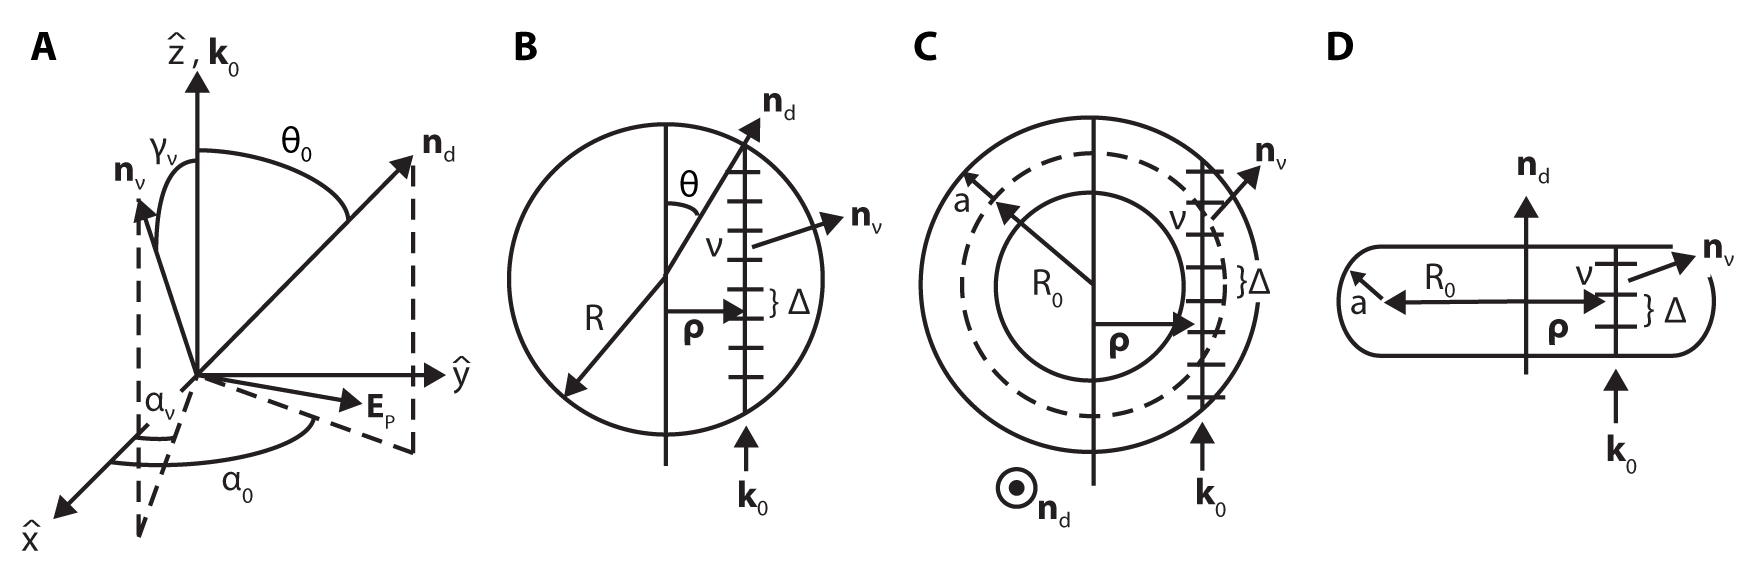
\includegraphics{figures/C4/Ch4-Figs_JonesGeometry.png}
\caption{Symbols and coordinates used in simulating OPM droplet textures.
(A), Relevant angles used in all simulations, where $\mathbf{n}_d$ is the droplet director, $\mathbf{n}_{\nu}$ is the local director, $\mathbf{k}_0$ is the incident wave vector, $\mathbf{E}_P$ gives the orientation of the polarizer.
$\mathbf{n}_d$ is specified by $\theta_0$ and $\alpha_0$, while $\mathbf{n}_{\nu}$ is specified by $\gamma_{\nu}$ and $\alpha_{\nu}$, where $\theta_0$ and $\gamma_{\nu}$ are measured from $\hat{z}$ and $\mathbf{k}_0$, respectively, and $\alpha$ is measured off of $\hat{x}$.
(B), Breakdown of OPM simulation parameters in a spherical geometry, where $\bm{\rho}$ is the position vector in the final image and $\Delta$ is the thickness of the voxels used in the simulation.
(C,D), Breakdown of OPM simulation parameters in a torus viewed from the (C) side and from the (D) top.}\label{f:4-generalcoords}
\end{figure}

To find the intensity at a given point $I(\bm{\rho})$ in the simulated texture, with $\mathbf{\rho}$ the position vector in the texture, $\mathbf{E}_P$ is propagated along the ray $\mathbf{k}_0$ passing through $\bm{\rho}$.
To accomplish this, the Jones matrix and rotation matrices for every voxel encountered by $\mathbf{k}_0$ are applied to the initial polarization state to produce the final polarization state of the light leaving the nematic volume.
A schematic of this process for a spherical nematic volume can be seen in Figure \ref{f:4-generalcoords}(B).
Once we have propagated the polarization state through the nematic volume, we calculate $I(\bm{\rho})$ by passing the final polarization state through the analyzer and taking the magnitude squared of the result.
Writing $I(\bm{\rho})$ in terms of $\bm{\Theta}$ and $\mathbf{R}(\alpha)$:
\begin{align}
I(\bm{\rho}) &= |\bm{\Theta}_A \mathbf{R}(\alpha_A)\, \bm{\vartheta}(\bm{\rho}) \, \mathbf{E}_P|^2, \, \label{e:4-Intensity}
\end{align}
where
\begin{align}
        \bm{\vartheta}(\bm{\rho}) &=  \prod\limits_{\nu = 1}^{N(\bm{\rho})}
        \!\mathbf{R}(-\alpha_{\nu}(\bm{\rho})) \bm{\Theta}_{\nu}(\bm{\rho}) \mathbf{R}(\alpha_{\nu}(\bm{\rho}))\,, \label{e:4-general_operator_one}
\end{align}
and $\bm{\Theta}_A \mathbf{R}(\alpha_A)$ is the operator and associated rotation accounting for the analyzer angle, $\alpha_A$.
Taking advantage of the associative property of matrix multiplication and the fact that the product of two rotation matrices is the rotation matrix of the sum of the angles, we can re-write Eq.~\ref{e:4-general_operator_one} as:
\begin{equation}
\bm{\vartheta}(\bm{\rho}) =  \mathbf{R}(-\alpha_{N}(\bm{\rho}))
 \prod\limits_{\nu = 2}^{N(\bm{\rho})}
 \!\Big \{ \bm{\Theta}_{\nu}(\bm{\rho}) \mathbf{R}(\alpha_{\nu}(\bm{\rho})-\alpha_{\nu-1}(\bm{\rho})) \Big \}
 \bm{\Theta}_{1}(\bm{\rho}) \mathbf{R}(\alpha_{1}(\bm{\rho}))\,
\end{equation}

Therefore, the overall process to simulate an OPM texture from a given director field is: (i) discretize the volume into voxels such that the local director for each voxel can be considered constant, (ii) use the local director to calculate the angles $\gamma$ and $\alpha$ for each voxel, (iii) use $\gamma$ and $\alpha$ to determine the Jones matrix and rotation matrix associated with each voxel, (iv) propagate the inital polarization state through the series of rotation matrices and Jones matrices, and (v) run the final polarization state through the analyzer and square the magnitude of the output to obtain the final intensity at every point.
This results in the OPM texture for a single wavelength.
To simulate a texture using multiple wavelengths, we average the different single-wavelength textures together.
\begin{figure}
\centering
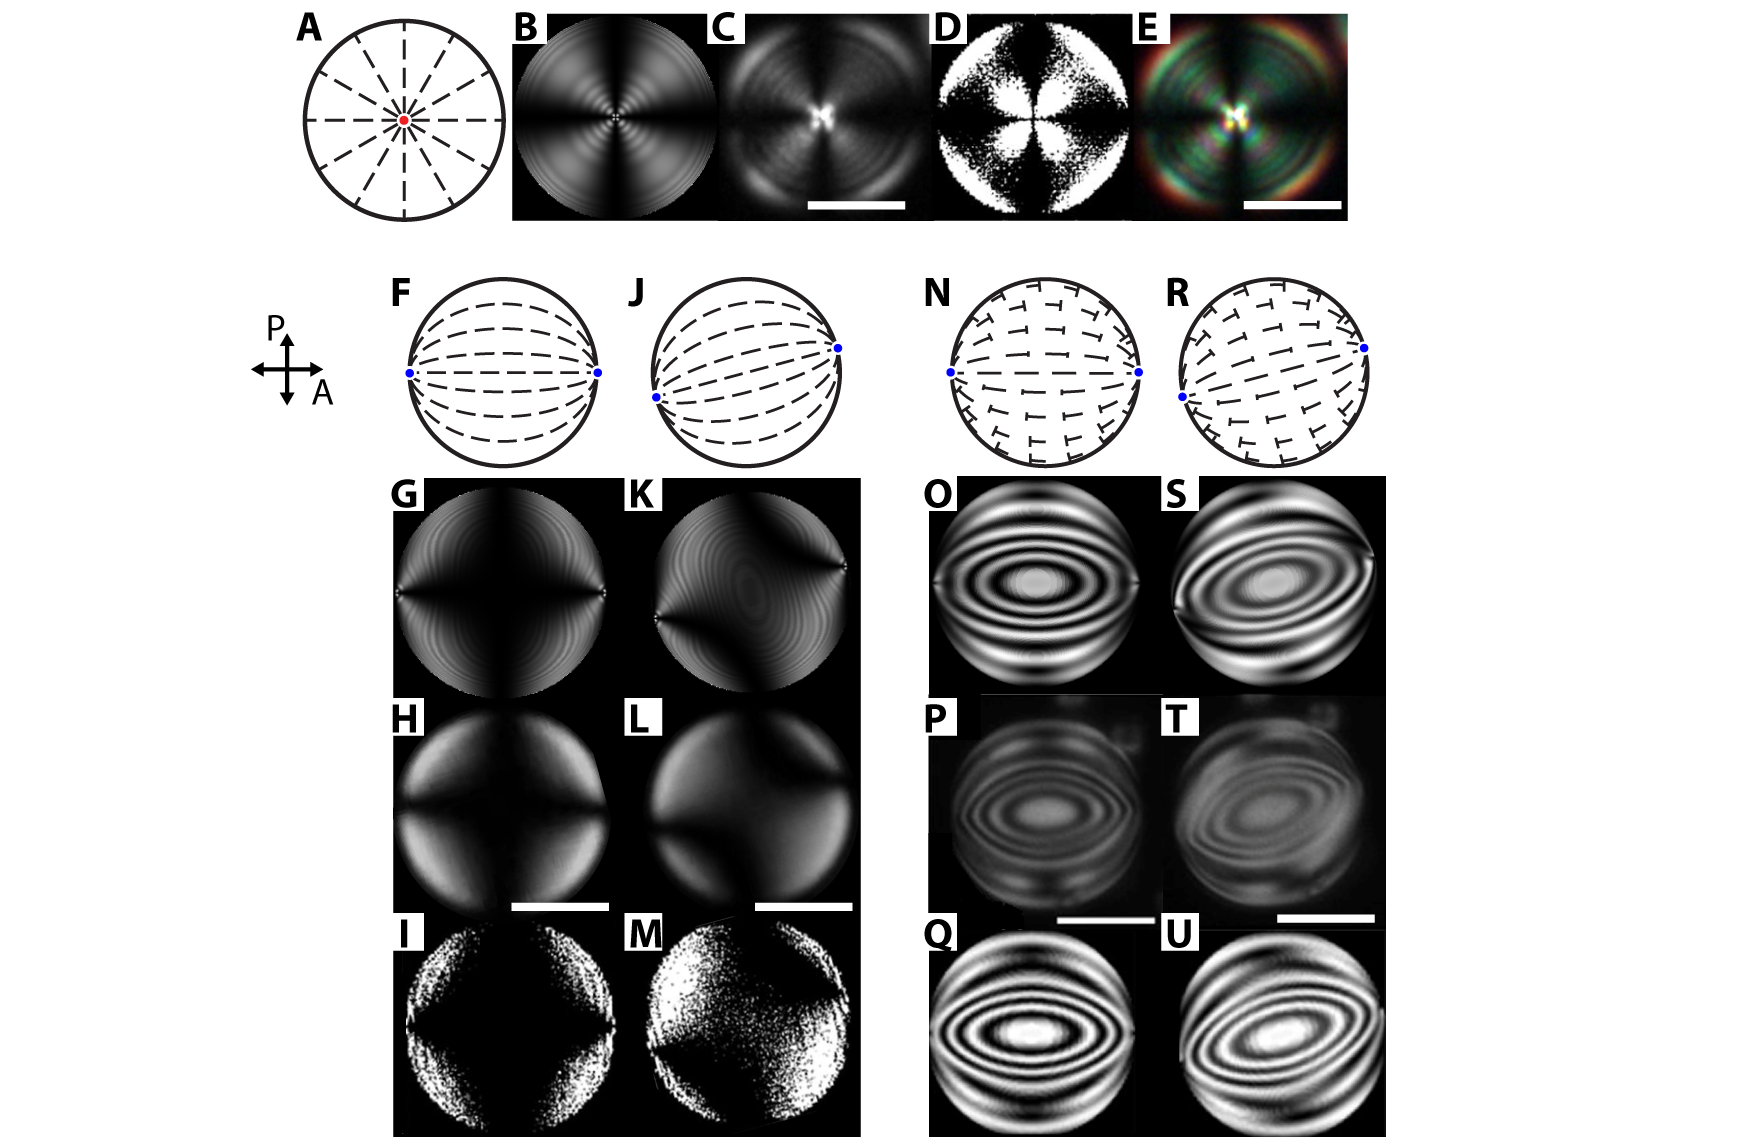
\includegraphics{figures/C4/Ch4-Figs_JonesSphere.png}
\caption{Director schematics and simulated and experimental OPM textures for (A--E) radial droplets, (F--M) bipolar droplets, and (N--U) twisted bipolar droplets.
For the radial droplets, (A) is a director schematic, (B) is a our simulation, (C,E) are a grayscale and color experimental image, respectively, and (D) is a simulation image from Ref.~\cite{RN310}.
For the bipolar and twisted bipolar droplets, (F--I) and (N--Q) are oriented with the bipolar axis aligned parallel to the analyzer direction while (J--M) and (R--U) have the bipolar axis rotated 15 degrees CCW from the analyzer direction. (F,J,N,R) are the schematics, (G,K,O,S) are our simulated images, (H,L,P,T) are experimental images, and (I,M,Q,U) are simulated textures from the literature.
(I,M) are from Ref.~\cite{RN310}, (P,T,Q,U) are from Ref.~\cite{RN193}.
Scale bar is 20 $\upmu$m in all images.
Images from Ref.~\cite{RN310} reprinted with the permission of AIP Publishing.
}\label{f:4-spherecomparison}
\end{figure}

\subsection{Validation using spherical droplets}
To test this method, we simulated OPM textures for the well-studied radial, bipolar, and twisted-bipolar director fields in spherical geometries.
For a radial director field we used $\mathbf{n}^{rad} = (x,y,z)/\sqrt{x^2+y^2+z^2}$~\cite{RN232}.
A simulated texture of a 40~$\upmu$m~diameter sphere calculated using $20$ evenly-spaced wavelengths between $400$~nm and $700$~nm is shown in Figure~\ref{f:4-spherecomparison}(B).
We compare our simulated image both with a grayscale experimental image of a 40~$\upmu$m~diameter 5CB droplet in water with 8 mM SDS and with another simulated texture of a $10$~$\upmu$m~diameter sphere from Ref.~\cite{RN310}.
These are shown in Figure~\ref{f:4-spherecomparison}(C,D), respectively.
The image in Figure~\ref{f:4-spherecomparison}(C) was converted to grayscale from the RGB image in Figure~\ref{f:4-spherecomparison}(E) using MATLAB's \texttt{rgb2gray} algorithm: $\mathit{gray} = 0.299 R + 0.587 G + 0.114 B$, where $R,G,B$ are the intensities in the red, green, and blue channels, respectively.
The conversion was done to better compare the simulated and experimental textures.

Note the agreement between our simulated image and the grayscale experimental texture; both show four dark, wedge-shaped brushes that begin in the center of the droplet and extend to the edges.
The bright portions also exhibit thin dark bands, or fringes, corresponding to locations where the retardation through the droplet is a multiple of $2 \pi$ for some or all of the wavelengths.
However, the experimental image is brighter in the center than our simulated image.
We attribute this difference to the defect not being in the focal plane in the experimental image; our simulated image does not take into account focus effects.
In addition, note how the bright portions of Figure~\ref{f:4-spherecomparison}(D) have a single, large, dark fringe where the retardation is a multiple of $2 \pi$.
The fringe in this simulated texture appears larger than those in Figure~\ref{f:4-spherecomparison}(B) because the simulated droplet here has a smaller size, and because the simulation was done with a single wavelength.

For a bipolar director we use $\mathbf{n}^{bp} = \nabla \psi/|\nabla \psi|$, where
\begin{align}
\psi =& \frac{1}{\sqrt{(x-p_x)^2+(y-p_y)^2+(z-p_z)^2}} \nonumber \\
      -& \frac{1}{\sqrt{(x+p_x)^2+(y+p_y)^2+(z+p_z)^2}}, \label{e:4-bipolar_pot}
\end{align}
with $\mathbf{p} = R(\sin \theta_0\cos\alpha_0,\sin \theta_0\sin\alpha_0,\cos\theta_0) $, and $R$ the sphere radius.
The simulated bipolar OPM texture of a 40 $\upmu$m diameter sphere for this director field using 20 evenly-spaced wavelengths between $400$ nm and $700$ nm for $\theta_0 = \pi/2$ and either $\alpha_0 = 0$ or $\alpha_0 = \pi/12$ are shown in Figure~\ref{f:4-spherecomparison}(G,K), respectively.
Corresponding experimental images of a 40 $\upmu$m diameter 5CB droplet in water with $1\%$ polyvinyl alcohol to enforce tangential anchoring, as well as simulated images of a 40 $\upmu$m diameter sphere from Ref.~\cite{RN310} are shown in Figure~\ref{f:4-spherecomparison}(H,L) and Figure~\ref{f:4-spherecomparison}(I,M), respectively.
All six images exhibit excellent agreement.
Note how Figure~\ref{f:4-spherecomparison}(G--I) all have four bright portions at the edge of the droplet and how the bright regions show a greater horizontal separation than a vertical separation.
Note also how the central region is completely dark.
When the droplet orientation changes by $\pi/12$ as seen in Figure~\ref{f:4-spherecomparison}(K--M), the central region in all three textures ceases being completely dark and begins to connect the upper-left and lower-right bright regions.

For a twisted bipolar director $\mathbf{n}^{tb}$, we follow Ref.~\cite{RN177} and use:
\begin{equation}
\mathbf{n}^{tb} = \mathbf{n}^{bp}\cos\tau +\mathbf{n}^{conc}\sin\tau,
\end{equation}
where the concentric director is $\mathbf{n}^{conc} = (\sin \varphi,\cos \varphi,0)$, with $\varphi$ the polar angle measured off of the x-axis.
$\mathbf{n}^{bp}$ is the bipolar director derived from the normalized gradient of Eq.~\ref{e:4-bipolar_pot}, and $\tau = \tau_0\sqrt{x^2+y^2}/\sqrt{R^2-z^2}$ is a twist angle varying from $\tau=\tau_0$ at the surface of the sphere to $\tau=0$ at the bipolar axis [see Figure~\ref{f:4-spherecomparison}(N,R)]~\cite{RN177}.
Instead of generating OPM textures with different $\alpha_0$ and a fixed polarizer and analyzer orientation as with the bipolar OPM textures, here we keep $\alpha_0=0$ and vary the polarizer and the analyzer orientations to generate different views.
This makes the computation easier to perform.
The simulated twisted bipolar OPM textures shown in Figure~\ref{f:4-spherecomparison}(O,S) were produced for a 50~$\upmu$m~diameter sphere with a single wavelength at $\lambda = 650$~nm.
The simulated twisted bipolar images from Ref.~\cite{RN193} were also produced for a similar sphere with $\lambda = 650$~nm, as seen in Figure~\ref{f:4-spherecomparison}(Q,U).
The experimental images of $\approx 40$ $\upmu$m diameter droplets imaged using $\lambda \approx 650$~nm from Ref.~\cite{RN193} are shown in Figure~\ref{f:4-spherecomparison}(P,T).
As with the bipolar droplets, the six twisted bipolar textures also show remarkable agreement.
Note how the number and position of the fringes in Figure~\ref{f:4-spherecomparison}(O--Q) and Figure~\ref{f:4-spherecomparison}(S--U) are the same.
In addition, note that while the central region in the bipolar drops in Figure~\ref{f:4-spherecomparison}(G--I) is dark, the addition of a twist in the director field about the horizontal axis causes the central region in the twisted bipolar textures in Figure~\ref{f:4-spherecomparison}(O--Q) to be bright.
Even though 20 wavelengths were used for the bipolar textures and only a single wavelength was used for the twisted bipolar textures, this is a valid comparison to make; using more or fewer wavelengths for the bipolar texture would not brighten the center, and using more wavelengths in the twisted bipolar texture would not darken the central region.


\subsection{Planar-anchored nematic toroids}
We first used simulated OPM textures in our previous work with NLC toroids under degenerate planar boundary conditions~\cite{RN24}.
We observed the toroidal droplets from the top, shown in the OPM texture in Figure~\ref{f:4-PlanarTorusComparison}(A), and from the side, shown in the bright-field image in Figure~\ref{f:4-PlanarTorusComparison}(D) and the OPM textures in Figure~\ref{f:4-PlanarTorusComparison}(E,F).
Note how the central region in the side-view OPM textures [red dashed line, Figure~\ref{f:4-PlanarTorusComparison}(E,F)] is always bright regardless of the PA orientation.
The fact that this central region cannot be fully extinguished under crossed polarizers can be explained with the doubly-twisted director field ansatz in Eq.~\ref{e:4-planransatz}~\cite{RN24}.
Recall that the parameter $\omega$ determines the amount of twist in the director field and $g$ allows the director field to splay; $g$ also controls the $\theta$-dependence of the director field.
When $g = 0$, the $\theta$-dependence vanishes and the director field is like that in a cylinder with $\xi = \infty$.
As $g$ increases, the twist measured along $\theta = 0,\pi$ becomes larger than $\tau$, which is measured along $\theta = \pi/2, 3\pi/2$.
Note that $g=1$ corresponds to a splay-free configuration.
From minimizing the Frank-Oseen free energy, including saddle splay, for different values of the toroidal aspect ratio, $\xi = R_0/a$, we obtained values of $\omega$ and $g$~\cite{RN24}.
The values are plotted with the (${\color{red} \bullet}$) symbols and the (${\color{blue} \blacksquare}$) symbols in Figure~\ref{f:4-OmegaG}, respectively.
As $\xi$ decreases, $\omega$ increases and $g$ decreases corresponding to an increase in the twist deformation.
Note that $g = 1$ only for $\xi \approx 3$; the minimum energy configuration typically contains both splay and twist distortions.
\begin{figure}
\centering
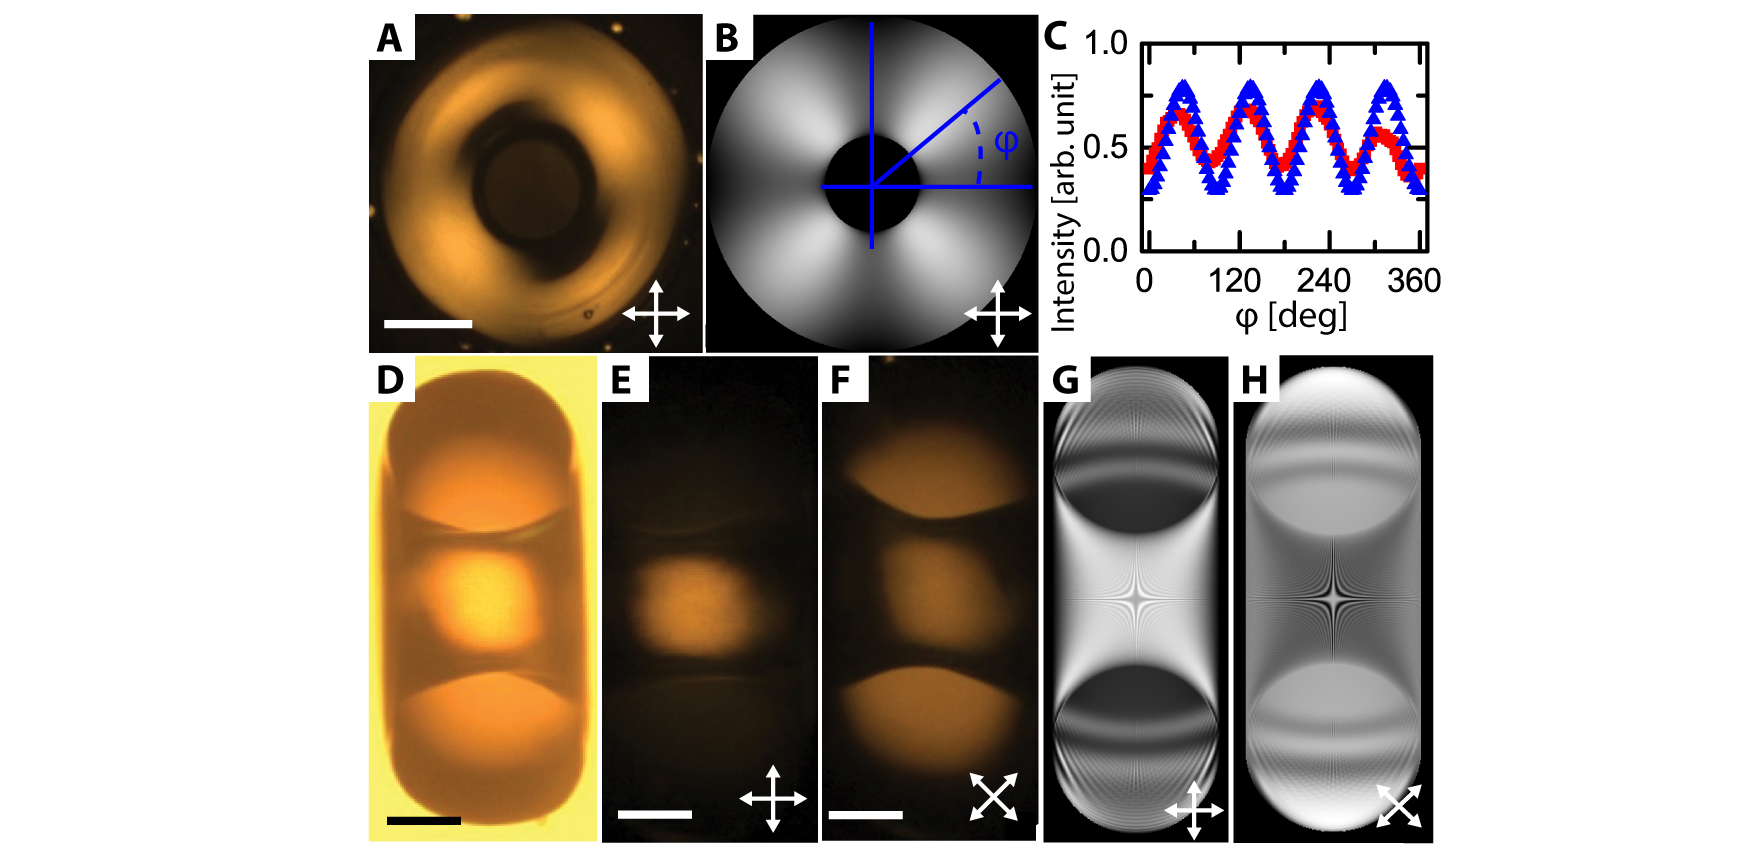
\includegraphics{figures/C4/Ch4-Figs_PlanarToroids.png}
\caption{Simulated OPM textures of nematic tori and experimental images of nematic toroids. (A,D--F), Experimental images of a tangentially-anchored nematic toroid with $\xi \approx 1.8$ from Ref.~\cite{RN24}.
(A), OPM view from the top, (D), bright field view from the side, and (E,F), OPM views from the side with PA oriented at $0^{\circ}$ and $45^{\circ}$, respectively.
(B,G,H), Simulated OPM textures for a torus of $\xi = 1.8$ using the ansatz from Eq.~\ref{e:4-planransatz} with $\omega= 0.420$ and $g=0.750$ from minimizing the free energy.
The OPM textures are viewed from the (B) top and from the side with P and A oriented at (G) $0^o$ and (H) $45^o$.
The intensity along the central ring for (A) ($\color{red}\blacksquare$) and (B) ($\color{blue}\blacktriangle$) is plotted in (C).
Scale bar is $100$ $\upmu$m in (E,F) and $200$ $\upmu$m in (A).}\label{f:4-PlanarTorusComparison}
\end{figure}

\subsubsection{Simulated textures}
We simulate OPM textures for nematic tori under tangential anchoring using the ansatz in Eq~\ref{e:4-planransatz} with values of $\omega$ and $g$ provided from the free energy minimization [see Figure~\ref{f:4-OmegaG}].
We produce textures using a weighted average over 200 wavelengths evenly-spaced between $400$ nm and $700$ nm.
The normalized weights are provided by approximating the spectrum of the tungsten lamp in the microscope used to take the experimental OPM textures~\cite{RN288}.
We use the functional form $\mathit{weight}(\lambda)  = \sqrt{(\lambda-375)/500} $, where $\lambda$ is in nm; after calculating the individual weights, we normalize them so that the sum of all the weights must equal to 1.
The normalized weights for 20 and 200 evenly-spaced wavelengths between 400 nm and 700 nm are plotted in Figure~\ref{f:4-Spectrum}, respectively.
We note that to better capture the output images, we could have also considered the spectral response of the camera in our experiments (The Imaging Source, DFK 41B02), plotted for the individual channels and the total luminance in Figure~\ref{f:4-CameraResponse}(A,B), respectively~\cite{camera}.
We simulate the side-view OPM texture by propagating the incident light perpendicular to $\mathbf{n}_d$, as seen in Figure~\ref{f:4-generalcoords}(C), and we simulate the top-view OPM texture by propagating the light along $\mathbf{n}_d$, as seen in Figure~\ref{f:4-generalcoords}(D).
\begin{figure}
  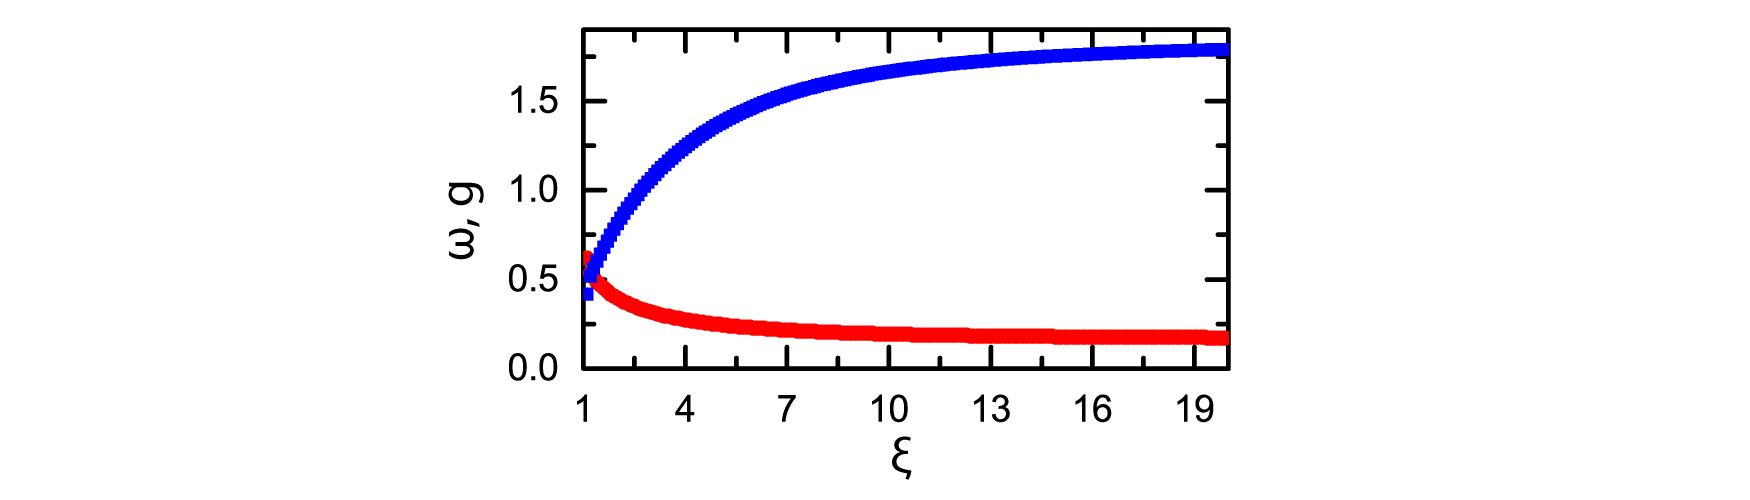
\includegraphics{figures/C4/Ch4-Figs_OmegaG.png}
  \caption{Values of ($\color{red} \bullet$) $\omega$ and ($\color{blue}\blacksquare$) $g$ as a function of $\xi$ obtained by minimizing the Frank-Oseen free energy for the ansatz in Eq.~\ref{e:4-planransatz}.}\label{f:4-OmegaG}
\end{figure}

Both the experimental top-view OPM texture in Figure~\ref{f:4-PlanarTorusComparison}(A) and the simulated top-view OPM texture in Figure~\ref{f:4-PlanarTorusComparison}(B) are predominantly bright with four brushes exhibiting partial extinction aligned along the polarizer and analyzer.
This can also be seen in $4$ maxima and $4$ minima in the intensity along the central ring from $\varphi=0^{\circ}$ to $\varphi=360^{\circ}$ as plotted in Figure~\ref{f:4-PlanarTorusComparison}(C) for the experimental OPM texture ($\color{red}\blacksquare$) and the simulated OPM texture ($\color{blue}\blacktriangle$).
In the simulations, the grayscale intensity goes from $0$ to $1$, corresponding to white and black in the simulated textures, respectively.
Note that the incident intensity is always $1$ in the simulations; for example, a value of $0.5$ in Figure~\ref{f:4-PlanarTorusComparison}(C) corresponds to half the incident intensity.
The two curves agree with respect to both the position of the minima and maxima and the relative height of the minima and maxima.
Note that the lack of complete extinction in the brushes is reflected in the height of the minima in the intensity plot; this high minimum intensity is due to the doubly-twisted structure of the director field.
As with the bipolar and twisted bipolar spherical droplets, the presence of twist raises the minimum intensity in the simulated OPM texture of the toroidal droplets.
\begin{figure}
  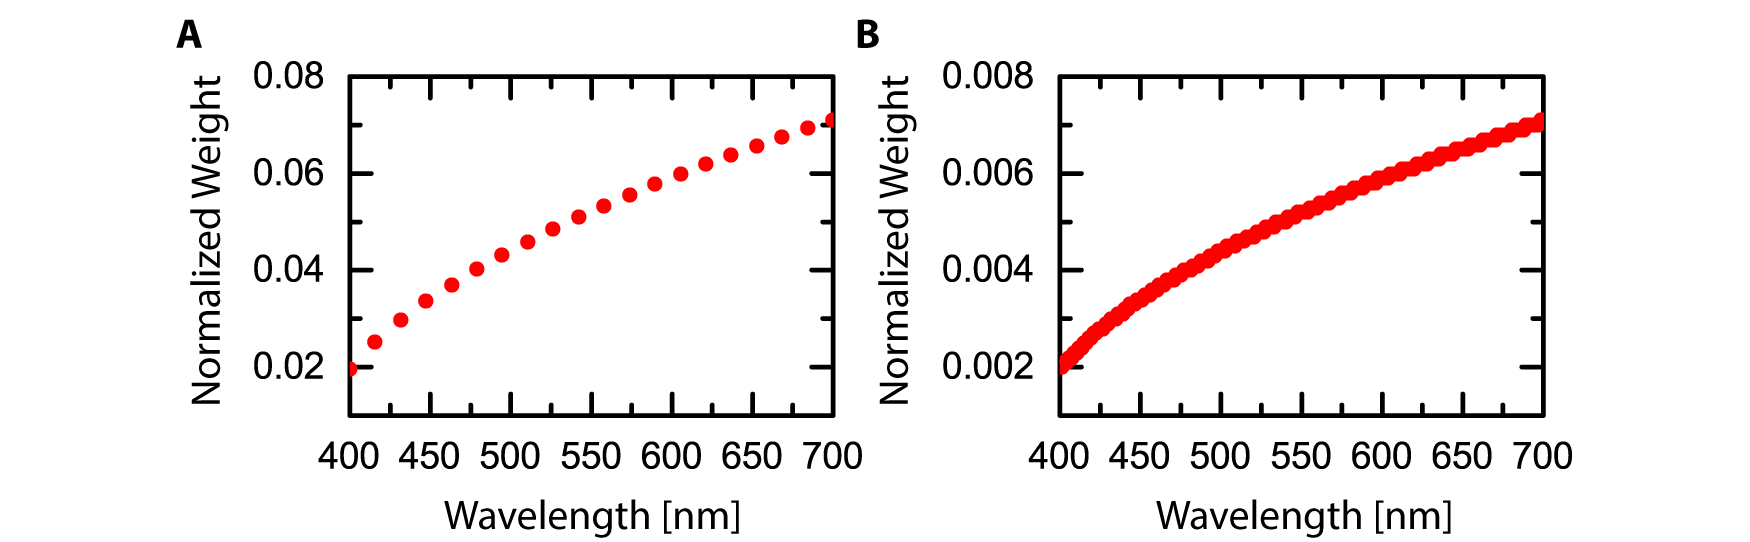
\includegraphics{figures/C4/Ch4-Figs_Spectrum.png}
  \caption{Normalized weights as a function of wavelength to approximate the spectrum of a tungsten lamp.
  (A,B), the weights for 20 and 200 evenly-spaced wavelengths between 400 nm and 700 nm, respectively.}\label{f:4-Spectrum}
\end{figure}
\begin{figure}
  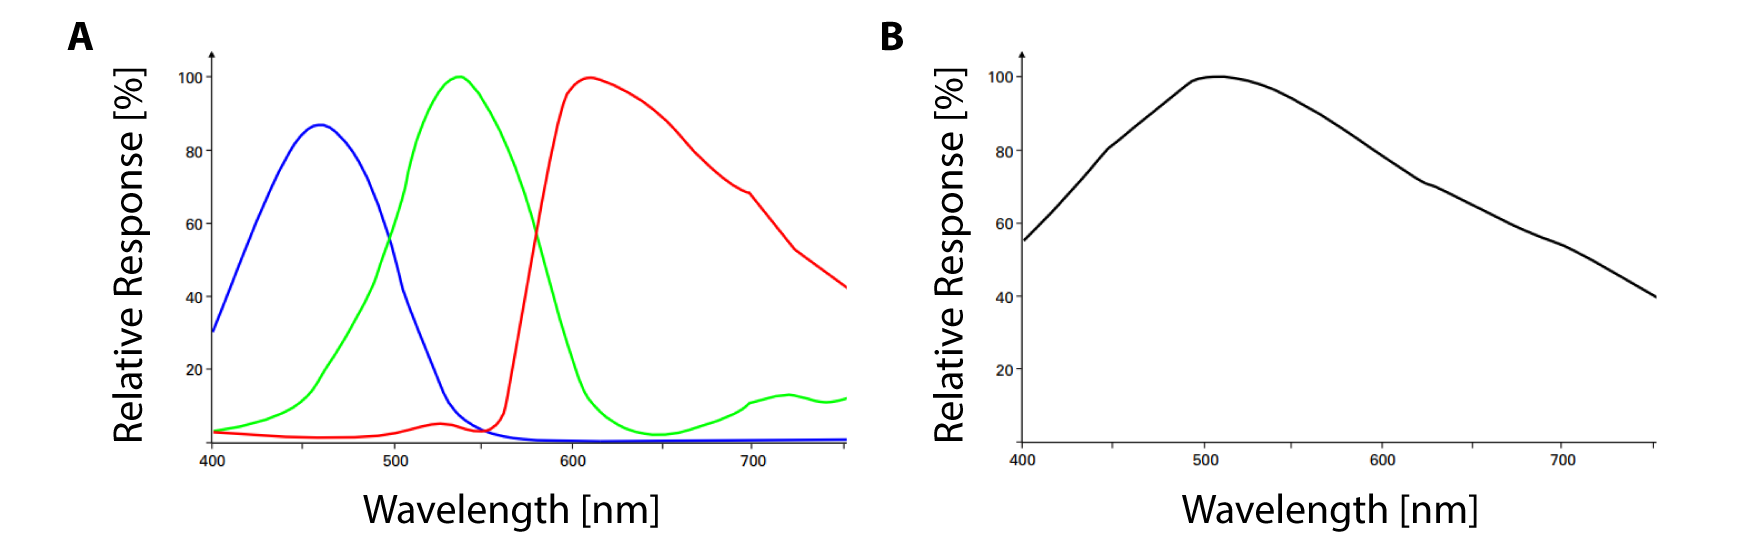
\includegraphics{figures/C4/Ch4-Figs_CameraResponse.png}
  \caption{Relative response for the sensor in our color camera (DFK 41BU02).
  (A,B), the (A) individual R, G, and B channel and (B) total luminance relative response as a function of wavelength~\cite{camera}.
  }\label{f:4-CameraResponse}
\end{figure}

The role of twist in preventing complete extinction is also present when looking at the brightness of the central region in both experimental side-view textures and the simulated side-view textures, as highlighted by the red dashed lines in Figure~\ref{f:4-PlanarTorusComparison}(E,F) and Figure~\ref{f:4-PlanarTorusComparison}(G,H), respectively.
In addition, we see that the central region of both the experimental and simulated textures viewed with P and A aligned at $0^{\circ}$ and $90^{\circ}$, respectively, measured with respect to $\mathbf{n}_d$ [Figure~\ref{f:4-PlanarTorusComparison}(E,G)], is brighter than when P and A are aligned at $45^{\circ}$ and $135^{\circ}$, measured with respect to $\mathbf{n}_d$ [Figure~\ref{f:4-PlanarTorusComparison}(F,H)].
Now looking at the inner portion of the tubes, indicated by the cyan dashed lines in Figure~\ref{f:4-PlanarTorusComparison}(E--H), we see that again for both experiment and simulation with P and A at $0^{\circ}$ and $90^{\circ}$ [Figure~\ref{f:4-PlanarTorusComparison}(E,G)], the intensity is less than when P and A are at $45^{\circ}$ and $135^{\circ}$ [Figure~\ref{f:4-PlanarTorusComparison}(F,H)].
\begin{figure}
\centering
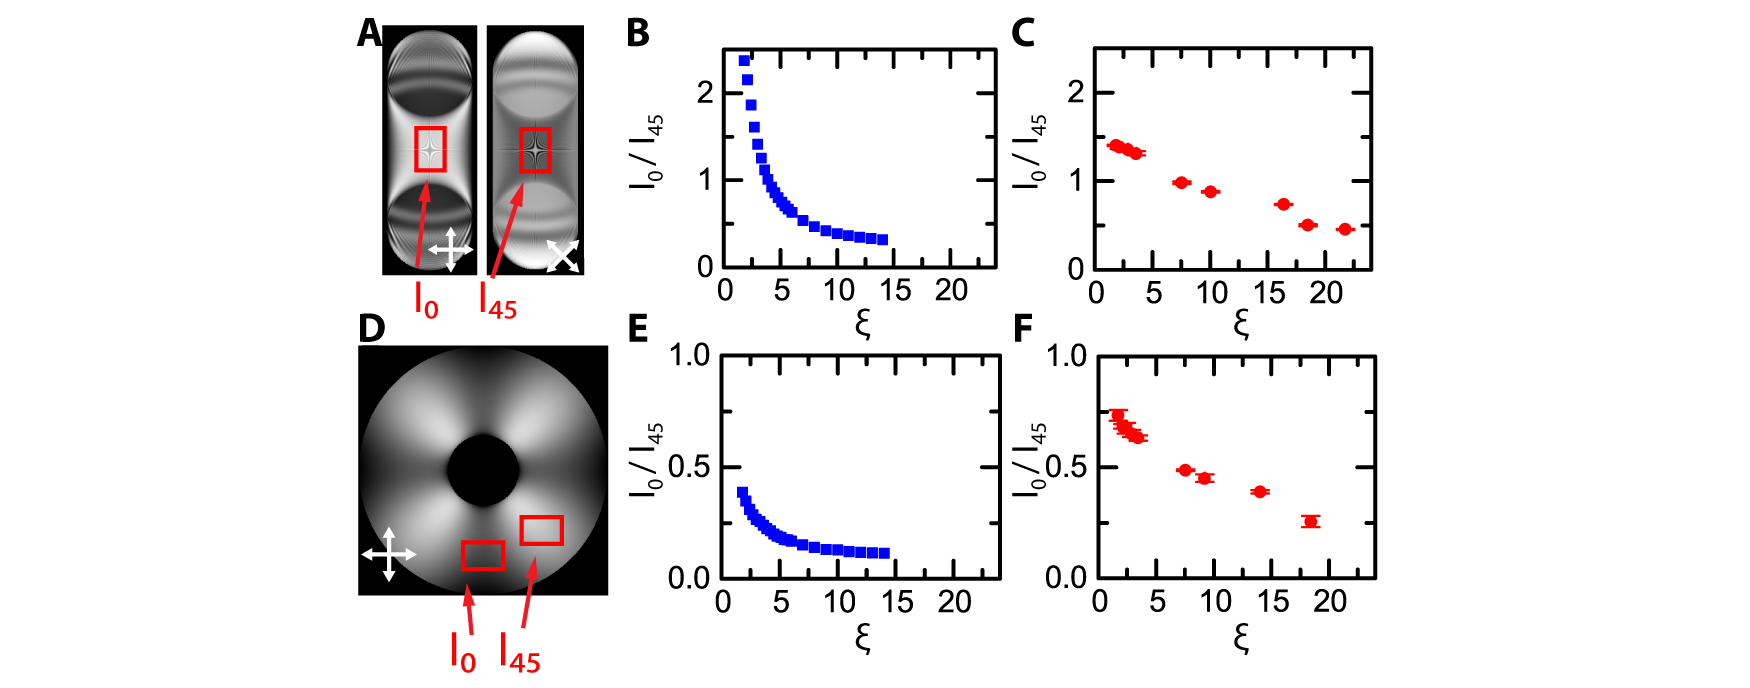
\includegraphics{figures/C4/Ch4-Figs_PlanarSimIntRat.png}
\caption{Intensity ratios for side-view and top-view simulated OPM textures of planar NLC toroids.
(A), Schematic detailing the $I_0$ and $I_{45}$ measurements from the side-view.
(B,C), $I_0/I_{45}$ versus $\xi$ for (B) simulated and (C) experimental OPM textures from the side-view.
(D) Schematic detailing the $I_0$ and $I_{45}$ measurements from the top-view.
(E,F), $I_0/I_{45}$ versus $\xi$ for (E) simulated and (F) experimental OPM textures from the top-view. }\label{f:4-PlanarIntRatio}
\end{figure}

We quantify the difference between the brightness of the central region of a side-view OPM texture when P and A are aligned at $0^{\circ}$ and $90^{\circ}$ ($I_0$) versus when P and A are aligned at $45^{\circ}$ and $135^{\circ}$ ($I_{45}$), as seen in Figure~\ref{f:4-PlanarIntRatio}(A), by taking the ratio of the two measurements $I_0/I_{45}$ as a function of $\xi$.
We find that for both the experimental and simulated OPM textures the intensity ratio decreases as $\xi$ increases. In addition, $I_0/I_{45}$ also passes through 1 around $\xi = 5$ for both the simulated and experimental textures, as seen in Figure~\ref{f:4-PlanarIntRatio}(B,C).
Physically, this corresponds to the aspect ratio where the entry director is oriented at approximately $67.5^o$ with respect to $\mathbf{n}_d$.
Thus the incident light at $0^{\circ}$ for the $I_0$ measurement and the incident light at $45^{\circ}$ for the $I_{45}$ measurement have the same angular difference from the entry director, yielding similar output polarization states, reflected by the fact that $I_0/I_{45} \approx 1$.
For $\xi \lesssim 5$, $I_0/I_{45} < 1$ the entry director is closer to $90^o$ measured from $\mathbf{n}_d$; here the angular difference between the entry director and the P and A direction is greater when P and A are along $45^{\circ}$ and $135^{\circ}$ than when P and A are along $0^{\circ}$ and $90^{\circ}$, corresponding to $I_{45}>I_0$.
When $\xi \gtrsim 5$, the opposite is true; the entry director is closer to $45^o$ measured from $\mathbf{n}_d$, leading to $I_{0}>I_45$ and $I_0/I_{45} > 1$.

For $I_0/I_{45}$ from the top-view OPM textures, we take the intensity in a region  $0^{\circ}$ measured from the polarizer axis for $I_0$ and the intensity in a region $45^{\circ}$ measured from the polarizer axis for $I_{45}$, as seen in Figure~\ref{f:4-PlanarIntRatio}(D).
As with the intensity ratio for the side view, $I_0/I_{45}$ for the top view also decreases with increasing $\xi$. However, $I_0/I_{45}<1$ always for the top view.
This is due to the fact that there is no aspect ratio where the entry director at $0^{\circ}$ and at $45^{\circ}$ possess the same angular difference from the incident direction of polarization.
The angular difference between the director at $0^{\circ}$ and the P and A orientation is always less than the angular difference between the director at $45^{\circ}$ and the P and A orientation.
This implies that $I_0 < I_{45}$ always, and is reflected in the fact that $I_0/I_{45}<1$ always for the top view.
For both the top view and the side view, the $I_0/I_{45}$ from the experimental textures shows good qualitative agreement with the $I_0/I_{45}$ from the simulated textures.
The decrease in $I_0/I_{45}$ as $\xi$ increases can be explained with the decreasing value of $\omega$.
As $\omega$ decreases, the twist decreases and the entry director will be more aligned along P and A when P and A are at $0^o$ and $90^o$ than when P and A are at $45^o$ and $135^o$.
This causes $I_0$ to decrease and $I_{45}$ to increase, such that $I_0/I_{45}$ decreases.
\begin{figure}
\centering
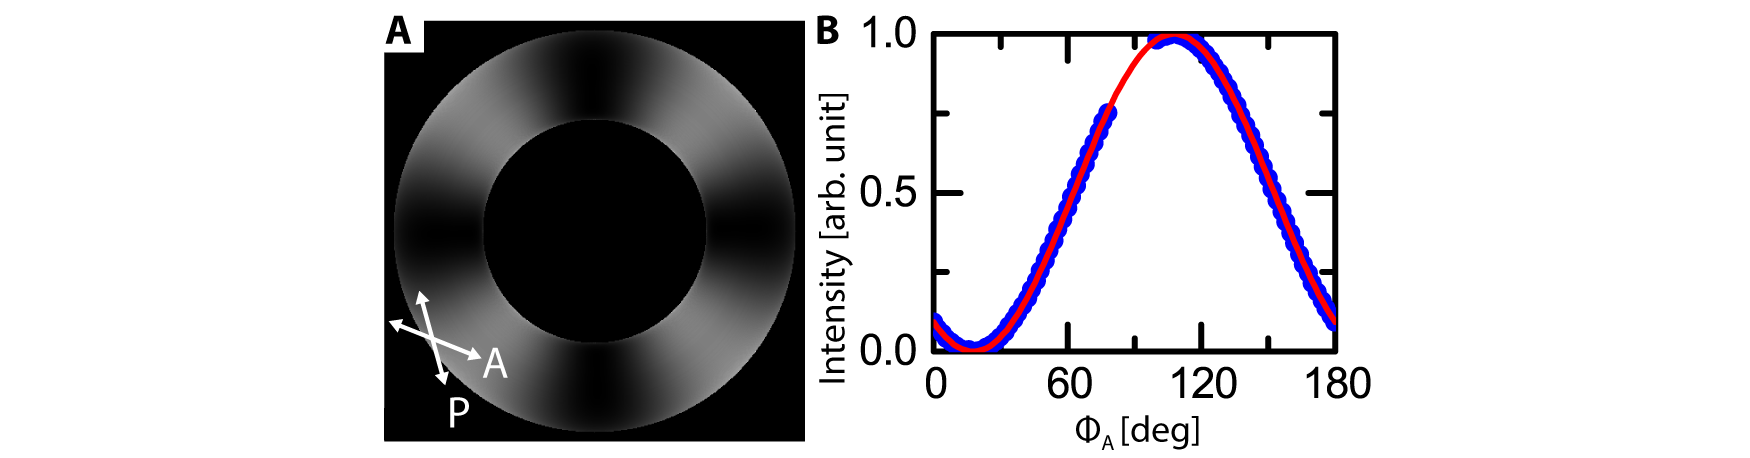
\includegraphics{figures/C4/Ch4-Figs_MeasuredTwist.png}
\caption{Predicted and measured twist angles for simulated OPM textures for planar NLC tori viewed from the top.
(A) Simulated texture with the polarizer and analyzer aligned to extinguish both the e-mode (dark regions aligned vertically) and the o-mode (dark regions aligned horizontally).
(B) Transmitted intensity as a function of analyzer angle with respect to the polarizer aligned along the entry director, with $1$ corresponding to complete transmission and $0$ to no transmission.
The fit is to the theoretical transmitted intensity for a twisted nematic cell in the waveguiding limit~\cite{RN232}.}\label{f:4-PlanarTwist}
\end{figure}

We now validate the relation between $\omega$ and the twist angle in our simulations.
Recall that the total twist angle of the director ansatz through the central ring viewed from the top can be written as $\tau = 2 \arcsin (\omega)$.
As an example, for $\xi = 3.5$, minimizing the free energy yields $\omega = 0.294$ and $g = 1.162$, corresponding to a theoretical $\tau = 34.2^{\circ}$.
We can confirm this by measuring the twist angle using simulated textures for $\xi=3.5$ with various P and A orientations.
We ``rotate'' the polarizer with a fixed A until the intensity at the central ring at $\varphi=0^{\circ}$ is a minimum, signifying that we have matched the polarizer orientation with the entry director.
We then fix P at this orientation and fit the intensity at $\varphi=0^{\circ}$ at the central ring as a function of analyzer angle to the expected transmission for a twisted nematic cell~\cite{RN232}:
\begin{align}\label{e:4-tn}
T = \cos ^2&(\Phi_{\textrm{exit}}-\tau)-\frac{\tau}{2 X}\sin(2X)\sin(2\Phi_{\textrm{exit}}-2\tau)\nonumber \\
&-\tau ^2\frac{\sin ^2 (X)}{X^2}\cos(2\Phi_{\textrm{exit}}-2\tau),
\end{align}
where $X = \sqrt{\tau^2+(\pi(n_E-n_o)d/\lambda)^2}$, $d$ is the sample thickness and $\Phi_\textrm{exit}$ is the angle of the analyzer measured with respect to the polarizer.
This fit for the example torus in Figure~\ref{f:4-PlanarTwist}(A) is shown in Figure~\ref{f:4-PlanarTwist}(B) and results in $\tau=33.61 \pm 0.01^{\circ}$.
This is consistent with our expectations from the theoretical ansatz and supports our simulation procedure.

Experimentally, we measured $\tau \approx 50^{\circ}$ for a toroid with $\xi \approx 3.5$~\cite{RN24}. Eq.~\ref{e:4-tn} assumes that the Mauguin parameter $u =  \pi (n_E-n_o) d /(\lambda \tau) \gg 1$~\cite{RN232}.
 Physically, this corresponds to a regime where the phase difference introduced by the birefringence is much greater than $\tau$ such that the nematic acts as a waveguide.
For our tori using 5CB with tube radius $\approx 100$ $\upmu$m, $u\sim 10^{2}$, satisfying this limit.
Provided the incident polarization is either parallel to the entry director (e-mode) or perpendicular to the entry director (o-mode), the incident polarization state will be propagated along the director twist and exit either parallel to (e-mode) or perpendicular to (o-mode) the exit director~\cite{RN232}.
Thus, an analyzer oriented perpendicular to the exit director will extinguish the e-mode and pass the o-mode while an analyzer oriented parallel to the exit director will extinguish the o-mode while passing the e-mode.
This can be seen in the simulated OPM texture in Figure~\ref{f:4-PlanarTwist}(A), where the e-mode has been extinguished in the dark brushes aligned along the vertical and the o-mode has been extinguished in the dark brushes aligned along the horizontal.


\subsubsection{Wavelength dependence of simulated OPM textures}
Since the simulation algorithm only works for a single wavelength, an average of multiple single-wavelength OPM textures is needed to approximate a true white light source.
To illustrate this effect, we will use the central section of a side view simulated OPM texture of a torus with $\xi = 1.8$, as seen highlighted in the red square in Figure~\ref{fig_lambda}(A).
For the single-wavelength images shown in Figure~\ref{fig_lambda}(B--E), the output polarization state varies spatially, leading to spatial intensity variations in the final image once the output polarization state is passed through the analyzer.
The symmetry of the ansatz found in Eq.~\ref{e:4-planransatz} in a perfect torus results in the light and dark bands encroaching symmetrically to produce the star-like feature seen in the middle of each individual single-wavelength image.
Note how the light and dark bands are smallest in the simulated texture for $\lambda = 400 $~nm displayed in Figure~\ref{fig_lambda}(B) and largest in the simulated texture for $\lambda = 700$~nm displayed in Figure~\ref{fig_lambda}(E).
This is because the retardation $\Gamma = 2\pi(n_E-n_o)d/\lambda \sim 1/\lambda$~\cite{RN232}.
Thus, as the light and dark bands are of different sizes and occur with different frequencies, averaging over multiple single-wavelength textures can wash out their appearance.
Averaging over more wavelengths in the same range corresponds to a greater washing out of the light and dark bands.
This is shown in Figure~\ref{fig_lambda}(F--I), where we average over 4, 8, 20, and 200 evenly-spaced wavelengths between $400$~nm and $700$~nm, respectively.
Also note how the star-like feature does not average out as it is present in all the simulated single-wavelength images.
\begin{figure}
\centering
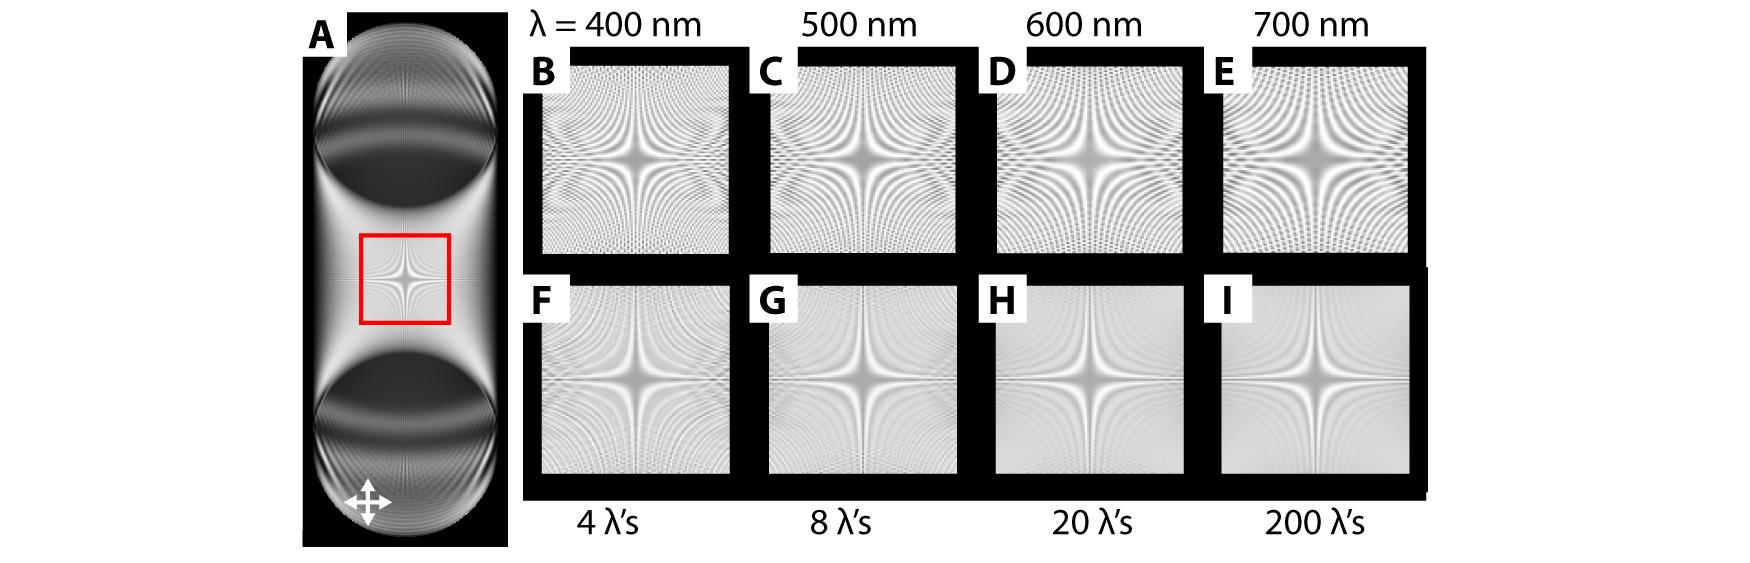
\includegraphics{figures/C4/Ch4-Figs_SimWavelengthAverage.png}
\caption{The effect of averaging over multiple wavelengths in a simulated OPM texture.
(A) Side-view simulated OPM texture of a planar NLC torus averaging over 200 wavelengths.
The red square highlights the central region shown in (B--I).
(B--E), The central region shown for the single wavelengths $400$~nm, $500$~nm, $600$~nm, and $700$~nm, respectively.
(F--I), The central region shown for an average of 4, 8, 20, and 200 wavelengths, respectively, over the interval $\lambda \in [400,700]$~nm.}\label{fig_lambda}
\end{figure}


\subsubsection{Effect of voxel size on simulated OPM textures}
The voxel size is important, as a voxel size too large will fail to capture the director variation in the volume, while a voxel size too small will take unnecessary time and computation power to simulate.
To capture the true effect of the given director field, the voxel must be small enough such that the director can be taken as a constant over the voxel volume.
Practically, this limit is found when simulating an OPM texture with a smaller voxel size produces no change in the output texture.
To illustrate this, the central portion of a side-view simulated OPM texture of a torus averaging over $200$ wavelengths are shown for P and A at $0^{\circ}$ and $90^{\circ}$ and at $45^{\circ}$ and $135^{\circ}$ in Figure~\ref{f:4-PlanarVoxel}(A--C) and Figure~\ref{f:4-PlanarVoxel}(D--F), respectively.
Comparing $\Delta /a = 0.04$ in Figure~\ref{f:4-PlanarVoxel}(A,D) with $\Delta /a = 0.01$ in Figure~\ref{f:4-PlanarVoxel}(B,E), we see that both the star feature and the fringes are much smoother when $\Delta /a = 0.01$ than when $\Delta /a = 0.04$.
In contrast, the difference between $\Delta /a = 0.01$ [Figure~\ref{f:4-PlanarVoxel}(B,E)] and the textures simulated for $\Delta /a = 0.001$ [see Figure~\ref{f:4-PlanarVoxel}(C,F)] is much less noticible.
Continuing to reduce the voxel size below $\Delta /a = 0.001$ produces no noticeable difference in the resulting textures.

While the individual textures show changes as $\Delta /a$ decreases towards $\Delta /a = 0.001$, the ratio $I_0/I_{45}$ over the central region of the simulated side-view OPM textures does not change, as seen in Figure~\ref{f:4-PlanarVoxel}(G) for $\Delta /a = 0.04$ ($\square$), $\Delta /a = 0.01$ (${\color{red}\square}$), and $\Delta /a = 0.001$ (${\color{cyan}\blacksquare}$).
All three curves fall on top of each other.
This is because $I_0/I_{45}$ is taken using the average intensity over the central region.
\begin{figure}
\centering
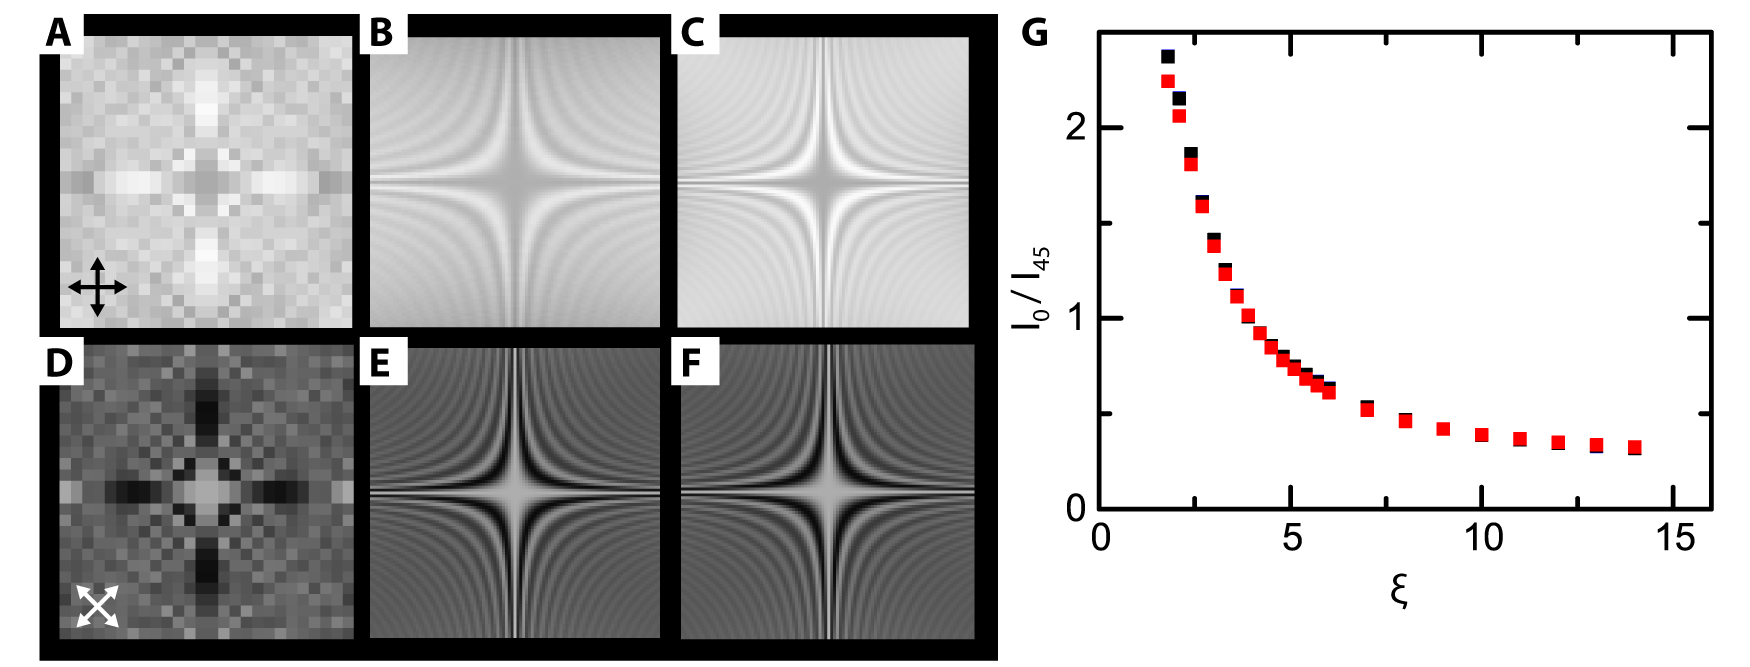
\includegraphics{figures/C4/Ch4-Figs_SimDeltaTest.png}
\caption{Effect of voxel size on individual OPM textures and on $I_0/I_{45}$ for planar NLC tori.
(A--F), The central region of a simulated side-view OPM texture with $\xi = 1.8$ with PA at $0^{\circ}$ (A--C) and PA at $45^{\circ}$ (D--F) for (A,D) $\Delta /a = 0.04$, (B,E) $\Delta /a = 0.01$, and (C,F) $\Delta /a = 0.001$.
All textures use a $200$ wavelength average with $a = 100$ $\upmu$m.
(G) Intensity ratio $I_0/I_{45}$ as a function of $\xi$ for simulated side-view OPM textures as seen schematically in Figure~\ref{f:4-PlanarIntRatio}(A) for ($\square$) $\Delta /a = 0.04$, (${\color{red}\square}$) $\Delta /a = 0.01$, and (${\color{cyan}\blacksquare}$) $\Delta /a = 0.001$.
}\label{f:4-PlanarVoxel}
\end{figure}

\subsubsection{Effect of refraction on OPM textures}
Even though the simulated OPM textures do not take into account refraction, refraction effects are present in the experimental textures and they affect how the experimental and simulated OPM textures can be compared.
First considering the experimental bright-field top view of an isotropic 5CB toroid with $n_{iso} \approx 1.6 $ in a yield-stress fluid with $n \approx 1.33$ in Figure~\ref{f:4-refraction}(A), the inner and outer edges of the torus are darker than the rest of the droplet.
In contrast, the inner and outer edges of the bright-field top view of a toroid made with polydimethylsiloxane (PDMS) oil with $n \approx 1.4$ in Figure~\ref{f:4-refraction}(B) are less prominent.
These effects of refraction are supported by simulated images of isotropic tori with $n = 1.4$ and $n = 1.2$ in an outer medium with $n=1$ seen in Figure~\ref{f:4-refraction}(C,D), respectively.
These images were generated by Ekapop Pairam using the 3D computer modeling software Autodesk Maya.
As with the experimental images, the simulated image with the higher index contrast is darker overall with more prominent edges than the image simulated with a smaller index contrast.
Thus, to minimize the effect of refraction on our data, we should only consider the region around the central ring when comparing simulated and experimental OPM textures for toroidal droplets viewed from the top.

We can also look at bright-field images of toroids viewed from the side made with either 5CB or PDMS oil immersed in a yield-stress medium, as seen in Figure~\ref{f:4-refraction}(E,F), respectively.
Viewed from the side, the central region and the inner portion of the tube of the 5CB toroid are bright, while the rest of the toroid is darker.
In contrast, the PDMS toroid viewed from the side has a fairly homogeneous intensity, with only the edges exhibiting some darkening.
As with the top view, these intensity trends are supported by simulated side-view images of tori with the higher index of refraction contrast shown in Figure~\ref{f:4-refraction}(G) and the lower index of refraction contrast shown in Figure~\ref{f:4-refraction}(H).
From these images, we find that we can only compare the central region and the inner portions of the tube between the experimental and simulated OPM textures of toroids viewed from the side.
\begin{figure}
\centering
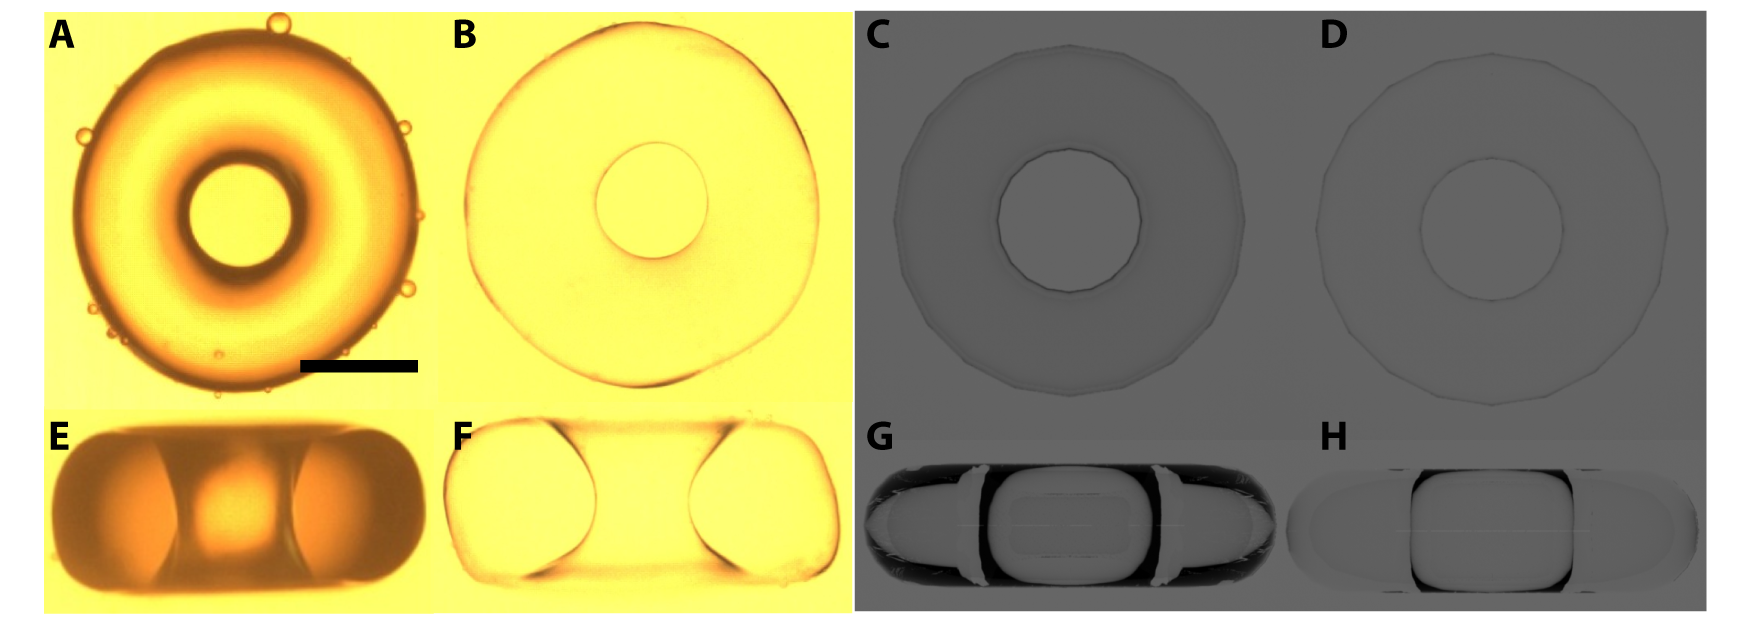
\includegraphics{figures/C4/Ch4-Figs_RefractionTest.png}
\caption{Effect of refraction of top and side view images of toroids.
(A,B,E,F), Experimental bright-field images of toroidal droplets of 5CB with (A,E) $n_{iso} \approx 1.6$, and (B,F) PDMS oil with $n \approx 1.4$ in a yield-stress outer medium with $n \approx 1.33$ viewed from the top (A,B) and from the side (E,F).
Scale bar for experimental images is $200$ $\upmu$m.
(C,D,G,H), Simulated bright-field images of isotropic tori with (C,G) $n =1.4$ and (D,H) $n=1.2$ with outer index of refraction $n = 1$ viewed from the top (C,G) and from the side (D,H).
Images simulated using Autodesk Maya.}\label{f:4-refraction}
\end{figure}

\subsubsection{The star feature in side-view simulated OPM textures of planar nematic tori}
While the general intensity trends agree, the simulated side-view OPM textures possess a star-like feature in the center that is not present in the experimental side-view OPM textures.
This feature does not affect the intensity measurements, as $I_0/I_{45}$ is calculated using the average intensity in the central region.
Given that the star feature is present in the single-wavelength images for $\lambda \in [400,700]$~nm with even a small voxel size of $\Delta/a = 0.0001$, the star is a real consequence of the director ansatz from Eq.~\ref{e:4-planransatz} confined to a perfect torus.
We further confirm this by simulating side-view OPM textures from truncated tori, where we truncate a torus by slicing the torus perpendicular to $\mathbf{k}_0$ at a truncation length $\ell_t$ measured along $\mathbf{k}_0$ from the end of the torus closest to the analyzer, as schematically shown in Figure~\ref{f:4-nostar}(D) for three truncation lengths.

For an example torus of $\xi=1.8$ and $a = 100$ $\upmu$m, we see that the star is present when simulating the OPM texture for the full torus with $\ell_t=0$ $\upmu$m [Figure~\ref{f:4-nostar}(A)], almost nonexistent when taking $\ell_t=10$ $\upmu$m [Figure~\ref{f:4-nostar}(B)], and is completely gone for $\ell_t=30$ $\upmu$m [Figure~\ref{f:4-nostar}(C)].
Changing the geometry from that of a perfect torus causes the star-like feature to disappear.
Since the experimental OPM textures come from toroids and not perfect tori, we believe that they do not have the symmetry required to exhibit a star-like feature in the center of their side-view OPM textures.
This is likely why we never observe such a feature in our experimental toroids.
\begin{figure}
\centering
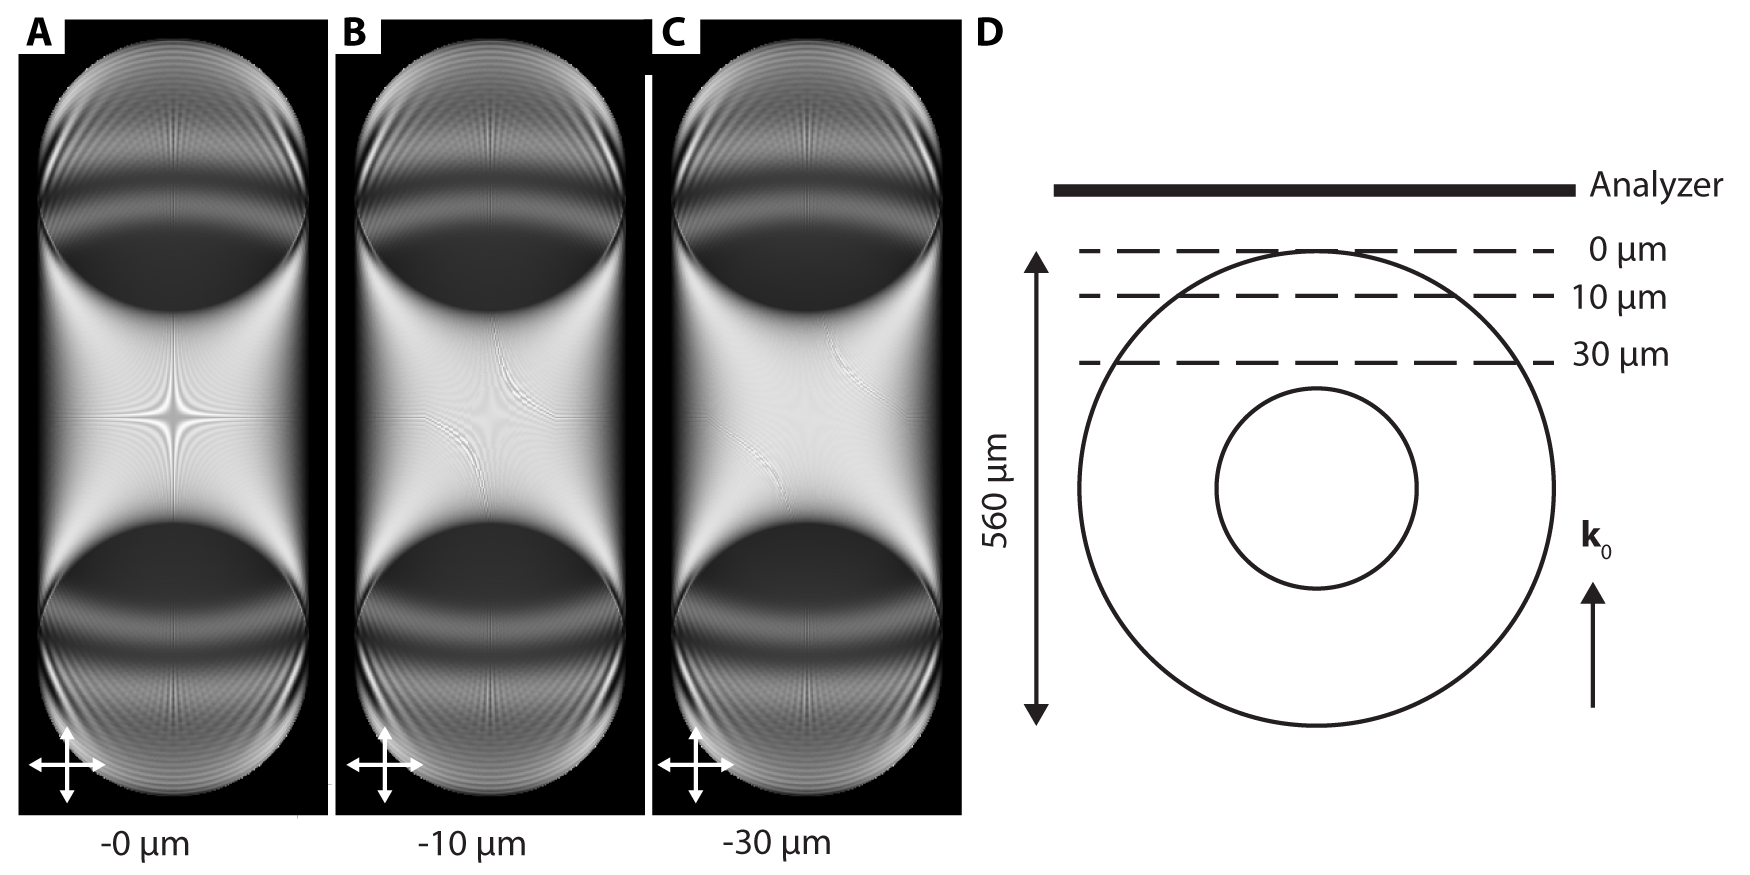
\includegraphics{figures/C4/Ch4-Figs_SimStarShape.png}
\caption{Effect of shape on the star feature in simulated OPM textures of planar NLC tori.
(A--C), Simulated OPM textures with $\xi = 1.8$ and $\Delta /a = 0.001$ for $a = 100$ $\upmu$m viewed from the side of truncated tori, as described schematically in (D).
All simulations performed averaging over 200 wavelengths.}\label{f:4-nostar}
\end{figure}


\subsection{Comparison with homeotropically-anchored nematic toroids}
We model a TER director field by coupling the doubly-twisted ansatz from our planar NLC toroids with the ER director field in the one-constant approximation:
\begin{equation}
  \mathbf{n} = \hat{r} \sin(\Omega)
  + \hat{\theta}\cos(\Omega)\frac{\omega r}{a- g \frac{r}{\xi} \cos \theta}
  + \hat{\varphi}\cos(\Omega)\sqrt{1 - \left ( \frac{\omega r}{a-g \frac{r}{\xi} \cos \theta} \right )^2 },\label{e:4-TERansatz}
\end{equation}
where $\Omega = 2 \arctan(r/a)$.
As with our simulated OPM textures of planar-anchored NLC toroids, we produce textures using a weighted average over 200 wavelengths evenly-spaced between $400$ nm and $700$ nm, where the weights are provided by the spectrum of the lamp in our microscope [see Figure~\ref{f:4-Spectrum}].
Comparing the example experimental TER texture in Figure~\ref{f:4-HomeoToroidsExp}(B) with the partial example simulated ER and TER textures in Figure~\ref{f:4-I0I45vsTwist}(A,B), respectively, we see that they share the same intensity features.
Both of the simulated textures and the experimental texture exhibit the classic dark-bright-dark-bright-dark pattern when $\varphi$ is aligned along the P and A directions.
This gives credence to our hypothesis that the director field in a homeotropic nematic toroid is either escaped-radial or twisted escaped-radial.
\begin{figure}
  \centering
  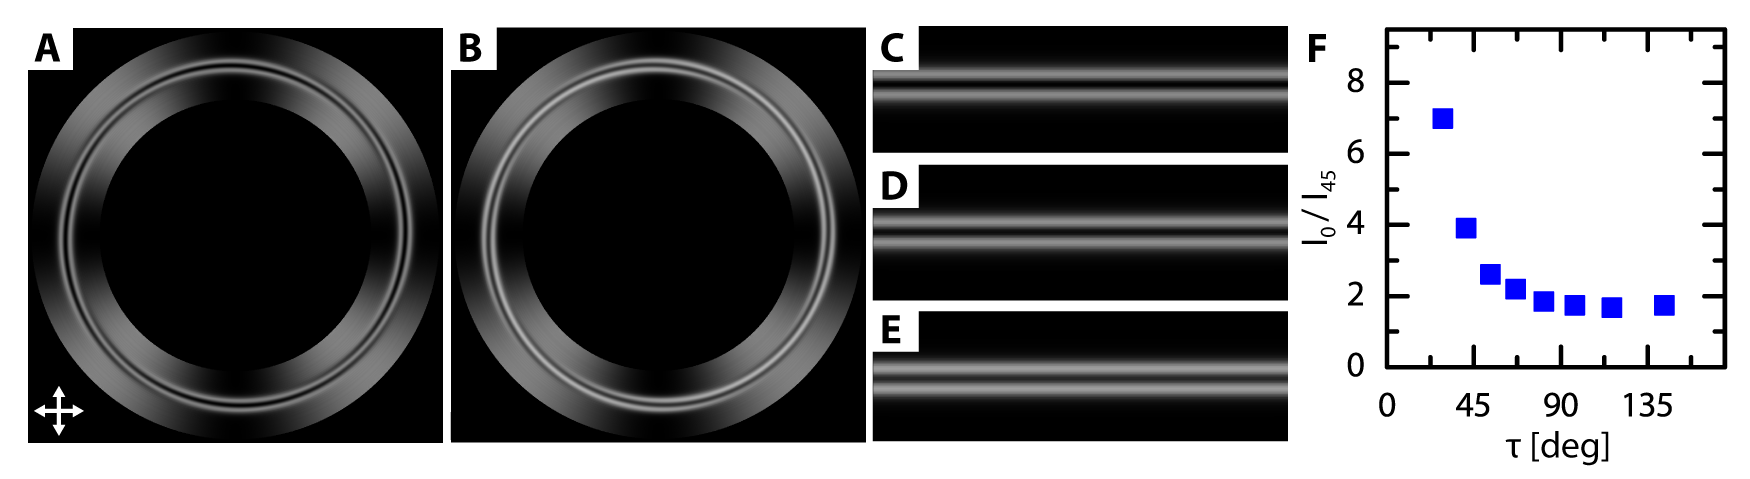
\includegraphics{figures/C4/Ch4-Figs_I0I45vsTwist.png}
  \caption{Simulated OPM textures, intensity profiles, and intensity ratios of TER configurations in tori and cylinders.
  (A--D), Simulated OPM textures of TER configurations in (A,B) tori and (C,D) cylinders.
  The textures are generated with twist angles (A,C) $\tau = 0^{\circ}$, (B,D) $\tau = 47.1^\circ$.
  (E), Intensity profiles from the simulated textures OPM textures in (A--D) corresponding to (${\color{blue} \square}$, ${\color{blue} \blacksquare}$, ${\color{red} \circ}$, ${\color{red} \bullet}$), respectively.
  (F), Intensity ratio vs twist angle for simulated TER OPM textures.}\label{f:4-I0I45vsTwist}
\end{figure}

To further confirm this, we simulate ER and TER capillaries, as shown in Figure~\ref{f:4-I0I45vsTwist}(C,D), respectively.
Here, we replace $\hat{\varphi}$ in Eq.~\ref{e:4-TERansatz} with $\hat{z}$, which we choose parallel to the capillary axis.
From the top, we first see that our simulated ER and TER textures in a [Figure~\ref{f:4-I0I45vsTwist}(A,B)] torus and simulated ER and TER textures in a [Figure~\ref{f:4-I0I45vsTwist}(C,D)] capillary have the same alternating dark and bright intensity features.
We plot the intensity profiles in the simulated OPM textures of the tori (${\color{blue} \square,\,\blacksquare}$) and the cylinders (${\color{red} \circ,\,\bullet}$) in Figure~\ref{f:4-I0I45vsTwist}(E).

Second, from this plot we see that the intensity profiles are geometry independent; provided the $\hat{\varphi}$ and $\hat{z}$ have the same $\tau$ and same orientation with respect to PA, the intensity profiles across the tube for the tori and the cylinders are identical.
Thus, as expected, ER/TER configurations in a torus can be recognized by the classic alternating light and dark pattern associated with ER/TER capillaries.
The TER configurations can further be distinguished from the ER configurations by the high central minimum in the TER intensity profiles [see Figure~\ref{f:4-I0I45vsTwist}].
Third, we see that the intensity profiles of the simulated ER textures [(${\color{blue} \square},{\color{red} \circ}$), Figure~\ref{f:4-I0I45vsTwist}(E)] in the tori and the cylinders have $I_{min} = 0$, in contrast to the experimental ER/TER textures in the capillaries; as mentioned earlier we believe that this is due to scattering from thermal fluctuations in the director orientation~\cite{RN33,RN309}
Thus, while we cannot make a quantitative comparison between the intensity profiles in the experimental and simulated ER/TER toroidal textures, we can use our simulated OPM textures to investigate how the twist affects a TER texture.


\subsection{Intensity ratio as a function of twist parameter}
We simulate TER configurations for varying $\omega$ in tori, measure the intensity profiles, and plot $I_{max}/I_{min}$ vs $\tau$ in Figure~\ref{f:4-I0I45vsTwist}(F).
We find $I_{max}/I_{min}$ varies inversely and monotonically with $\tau$.
This confirms our expectations that adding twist raises the intensity of the central minimum in an OPM texture of a TER director configuration, causing $I_{max}/I_{min}$ to decrease.
In addition, the monotonic relationship between the intensity ratio and $\omega$ implies that we can use $I_{max}/I_{min}$ as a proxy for twist.
Thus, our observation that  $I_{max}/I_{min}$ increases with $\xi$ [see Figure~\ref{f:4-HomeoToroidsExp}(G)] confirms that the amount of twist in a TER configuration in a toroid decreases with increasing $\xi$.
This suggests that geometry is the driving factor in generating a TER structure.
In addition, we argue that the twist in the TER structure results from bending the escape core, the central portion of the escape where $\mathbf{n} \sim \hat{\varphi}$.
This is similar to straight capillaries filled with SSY, where the twist distortion also relieves a bend distortion.
However, in SSY, $K_{11} \sim K_{33} \gg K_{22}$, such that it is energetically favorable to twist, even when the escape core is straight.
In our case, we use 5CB with $K_{11} \sim K_{22} \sim K_{33}$.
As a result, it seems that we need to introduce an extra bend distortion by bending the escape core to make the twist distortion energetically favorable in this case.


\subsection{Intensity ratio as a function of escape rate}
When we look closely at the escape core in the simulated TER textures in tori, we see that the escape core appears to spiral, similar to the experimental textures for NLC confined to toroids with low $\xi$.
To test if we can obtain a spiral texture in our simulations similar to that in the experiments by changing the escape rate, we modify the ER and TER ansatzes from Eq.~\ref{e:4-TERansatz} by taking $\Omega = (\pi/2)(r/a)^{\phi}$.
Recall that choosing $\phi = 1$ well approximates $2 \arctan(r/a)$, the one-constant solution [blue curve, Figure~\ref{f:4-EscapeSchem}(D)]; choosing $\phi < 1$ yields a slower escape [red curves, Figure~\ref{f:4-EscapeSchem}(D)]; and $\phi > 1$ yields a faster escape [red curves in Figure~\ref{f:4-EscapeSchem}(D)].

Observing textures and the intensity profiles for $\phi = 1,10,25$ in Figure~\ref{f:4-I0I45vsEscape}(A--C), respectively, we see $\phi > 1$ produces textures that qualitatively resemble those from our experimental toroids with the spiral textures.
However, when we plot $I_{max}/I_{min}$ vs $\phi$ for $\tau = 34.9^{\circ}$, we see that $\phi$ has no effect on the intensity ratio.
This indicates that the intensity ratio in the spiral textures is still only determined by the twist in the texture.
\begin{figure}
  \centering
  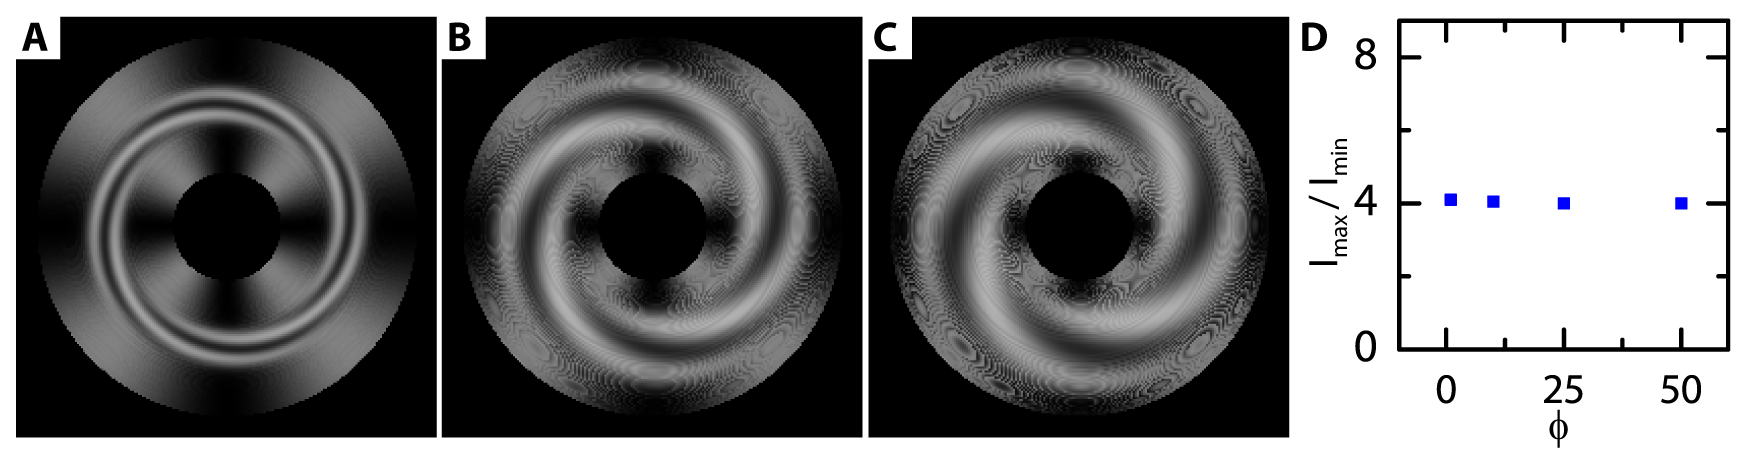
\includegraphics{figures/C4/Ch4-Figs_I0I45vsEscape.png}
  \caption{Simulated OPM textures and intensity ratios of TER configurations in tori with varying escape rates.
  (A--C), Simulated OPM textures of TER configurations with $\tau = 34^\circ$ and $\Omega = (\pi/2)(r/a)^{\phi}$, where (A) $\phi = 1$, (B) $\phi = 10$, and (C) $\phi = 25$.
  (D), Intensity ratio vs $\phi$ for OPM textures with $\tau = 34.9^\circ$.}\label{f:4-I0I45vsEscape}
\end{figure}

\section{Nematic liquid crystals in bent capillaries}
To test whether geometry is the underlying cause for observing a TER texture in homeotropic NLC toroids, we consider 5CB under homeotropic anchoring in bent glass capillaries.


\subsection{Making bent capillaries}
We start with straight glass capillaries, heat the glass at a point with a blowtorch, and let gravity bend the capillary such that the capillary axis now forms a planar curve, as seen in the bright-field image of an example capillary in Figure~\ref{f:4-BentCaps}(A).
We apply the heat for as short of a duration as possible to minimize the change in the inner diameter of the capillary; applying the torch over a long duration melts the capillary.
\begin{figure}
  \centering
  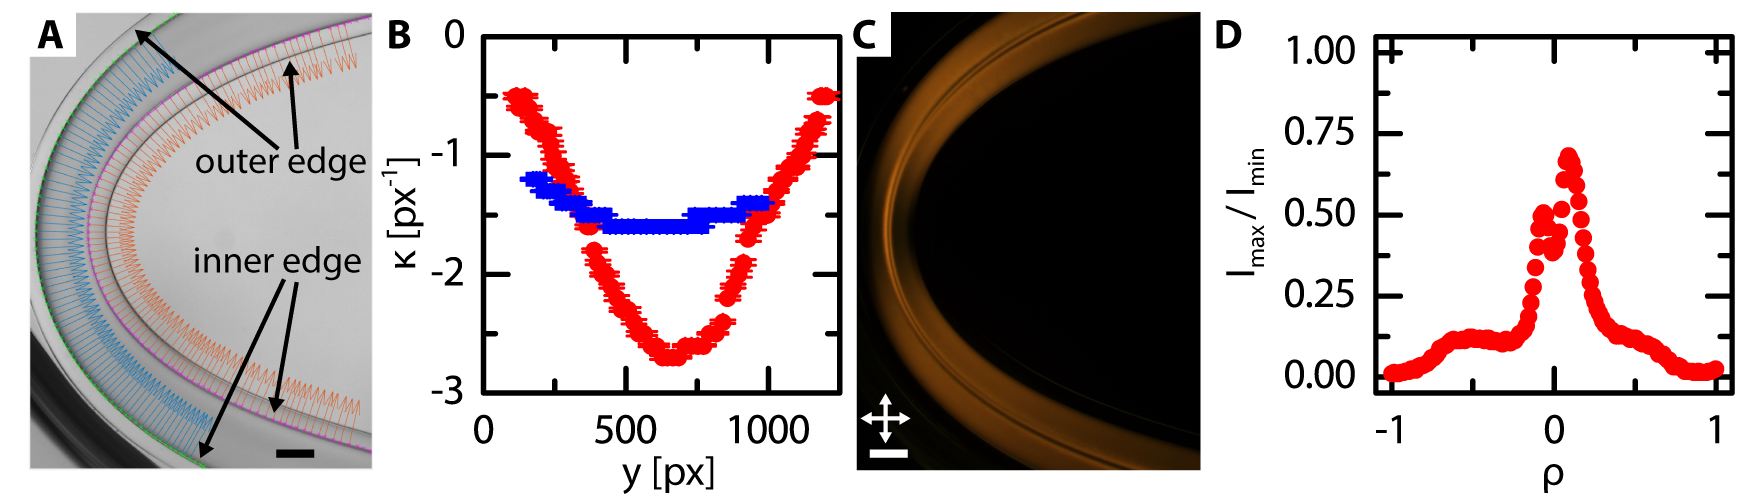
\includegraphics{figures/C4/Ch4-Figs_BentCaps.png}
  \caption{Measuring curvature and intensity profile in homeotropic NLC confined to bent capillaries.
  (A), Bright-field image of a bend capillary with points selected along the left and right contour.
  The normal vectors at each point are plotted on the image.
  (B), The measured curvature along the (${\color{blue} \blacksquare}$) left contour and (${\color{red} \bullet}$) right contour of the image in (A).
  (C), OPM image of the capillary in (A).
  (D), Intensity profile from the OPM texture in (C).
  For this profile, $I_{max}/I_{min} = 1.8$ and $\xi^{cap} = 6.8$.}\label{f:4-BentCaps}
\end{figure}

\subsection{Measuring planar curvature}
We measure the curvature of the capillary axis using a modified version of the IRLS routine we used in Chapter~\ref{c:3} to measure surface curvature.
Here, instead of fitting to the extended Weingarten Matrix, we fit to the Frenet-Serret formula, $\textrm{d}\mathbf{k}/\textrm{d}s = -\kappa \cdot \mathbf{T}$, where $s$ the arclength parameter, $\mathbf{T}$ the unit tangent vector, $\mathbf{k}$ the unit normal vector, and $\kappa$ the curvature~\cite{RN23}.
We then use:
\begin{equation}
  \Delta \mathbf{k} \cdot \mathbf{T} = \kappa \, \Delta s,\label{e:4-FSfit}
\end{equation}
with $\Delta s$ the independent variable, $\Delta \mathbf{k} \cdot \mathbf{T}$ the dependent variable, and $\kappa$ a fitting parameter.
This approach is equivalent to fitting to the Weingarten Matrix for a surface with only one nonzero principle curvature everywhere, i.e. a surface with vanishing Gaussian curvature but nonzero mean curvature.

For a planar curve, we choose points along the contour by hand and then estimate $\mathbf{T}$ and $\mathbf{k}$ by calculating finite differences as in Chapter~\ref{c:3}; these points and initial $\mathbf{k}$ are plotted for the left and right contour on the image in Figure~\ref{f:4-BentCaps}(A).
We initially estimate $\kappa$ for a point of interest by fitting Eq.~\ref{e:4-FSfit} for all pairs of points within $s_1$ neighbors of the point of interest, where we take $\Delta \mathbf{k}_{[i,j]} = \mathbf{k}_{[i]} - \mathbf{k}_{[j]}$ and $\Delta s_{[i,j]} \approx
\textrm{sign}\big \{ (\mathbf{r}_{[i]} - \mathbf{r}_{[j]}) \cdot \mathbf{T}\big \} |\mathbf{r}_{[i]} - \mathbf{r}_{[j]}|$.
We then use this initial estimate as the input for our IRLS routine and fit Eq.~\ref{e:4-FSfit} considering all pairs of points within $s_2$ neighbors of the point of interest.

For the example image in Figure~\ref{f:4-BentCaps}(A), we fit the left contour with $s_1 = 1$, $s_2 = 13$ and the right contour with $s_1 = 1$, $s_2 = 19$, plotting the output curvature [(${\color{blue} \blacksquare}$) left contour, (${\color{red} \bullet}$) right contour] in Figure~\ref{f:4-BentCaps}(B).

\subsection{Measuring the intensity profile}
To assign a local aspect ratio, we need the curvature along the central capillary axis.
To find this, we start by selecting a point of interest in the capillary near the central axis.
We then find the nearest point on the left and right contours, $\mathbf{p}_{left}$ and $\mathbf{p}_{right}$, and take the intensity profile along the line connecting $\mathbf{p}_{left}$ and $\mathbf{p}_{right}$.
The central ring radius for the intensity profile is then given by $R^{cap}_0 = (1/2)(\kappa(\mathbf{p}_{left}) + \kappa(\mathbf{p}_{right}))^{-1}$, and the tube radius $a^{cap} = |\mathbf{p}_{left} - \mathbf{p}_{right}|/2$, such that we can calculate the local aspect ratio $\xi^{cap} = R^{cap}_0/a^{cap}$.
Thus, we see that in a single bent capillary we can explore a variety of $\xi$ simply by changing the crossed P and A to align with the capillary axis along different portions of the capillary.
For the example OPM texture in Figure~\ref{f:4-BentCaps}(C), we plot the intensity profile in Figure~\ref{f:4-BentCaps}(D), where $\xi^{cap} = 6.8$.
Note that similar to the toroids and to the straight TER capillaries, the maxima in the intensity profile of the bent capillaries generally have different intensity values.
Since we observe no trend in which maximum is higher in the intensity profile, we employ the same strategy as earlier and take $I_{max}$ to be the average of the two maxima in the intensity profile; for the example in profile in Figure~\ref{f:4-BentCaps}(D), we find $I_{max}/I_{min} = 1.8$.


\subsection{Comparison with toroids}
We find that the intensity profiles for the $\xi^{cap} \rightarrow \infty$ regions of the bent capillary resemble the intensity profiles for the ER capillaries, while the intensity profiles with a finite $\xi^{cap}$ [Figure~\ref{f:4-BentCaps}(D)] have the raised central minimum indicative of a TER configuration, and similar to our TER toroids.
Plotting $I_{max}/I_{min}$ for the capillaries as a function of the local aspect ratio [($\blacktriangle$), Figure~\ref{f:4-HomeoToroidsExp}(G)] on top of our data from the homeotropic toroids [(${\color{blue} \circ}$), Figure~\ref{f:4-HomeoToroidsExp}(G)], we see that the data fall on top of each other, confirming that the amount of twist is determined solely by the local geometry.
From this perspective, $\xi$ can be seen as a dimensionless group locally comparing the relevant curvatures; $a$ gives the radius of curvature in the bend distortion inherent to an escaped radial configuration, while $R_0$ is the radius of curvature of the additional bend distortion induced by bending the capillary.
Bending the capillary breaks the symmetry of the bend distortion in the escape.
These two bend distortions do not compete in the same manner everywhere in the torus.
In particular, when $\theta = 0$, the two bend distortions are additive; when $\theta = \pi$, the two bend distortions are subtractive; and when $\theta = \pi/2,3\pi/2$ the two distortions are orthogonal.
The aspect ratio details the competition between the distortions: as $\xi$ decreases the competition between the distortions grows, and it becomes favorable to twist instead.


\section{Conclusions}
We have shown that geometry can affect the amount of twist in a homeotropic nematic confined to cylinders and toroidal droplets.
In addition, we see that for NLC that do not twist when confined to a volume with $\xi = \infty$, making $\xi$ finite can induce the nematic to twist, spontaneously breaking reflection symmetry in the process.
While this is similar to results in degenerate-planar anchored NLC toroids, in this case there is no explicit curvature-coupling in the free energy driving the reflection-symmetry breaking.
To show this, we relied on simulated OPM textures to relate the effect of twist in the director fired to the corresponding OPM textures.
We used planar-anchored toroids to demonstrate how the simulated textures responded to changing simulation parameters, and laid out a detailed methodology for simulating OPM textures in an arbitrary volume.

For NLC confined to a toroidal geometry with either homeotropic or degenerate planar boundary conditions, $\xi = R_0/a$ is the relevant geometrical parameter that controls the amount of twist in the system, comparing the scales of the relevant curvatures in the system.
Under degenerate-planar anchoring, $\xi$ is a measure of the difference between the principle curvatures, giving the strength of the saddle-splay distortion that drives the magnitude of the twist.
When the anchoring is homeotropic, $\xi$ instead gives the relative magnitudes of the bend distortions induced by the confinement; $a$ sets the scale of the bend distortion inherent in an ER configuration, $R_0$ sets the scale of the additional bend distortion induced by curving the capillary axis.
These distortions can compete; as the competition grows it becomes favorable to break reflection symmetry and twist, with the twist growing as to competition grows.
Since the aspect ratio can be defined locally, the twist in both anchoring scenarios can be adjusted by locally tuning the aspect ratio.
This demonstrates that confining NLC to toroidal-like geometries is a general strategy to tune chirality and investigate spontaneous symmetry breaking in an achiral material.
